\documentclass{article}
\usepackage{parskip}
\usepackage{pdfpages}
\usepackage[margin=.6in]{geometry}
\begin{document}
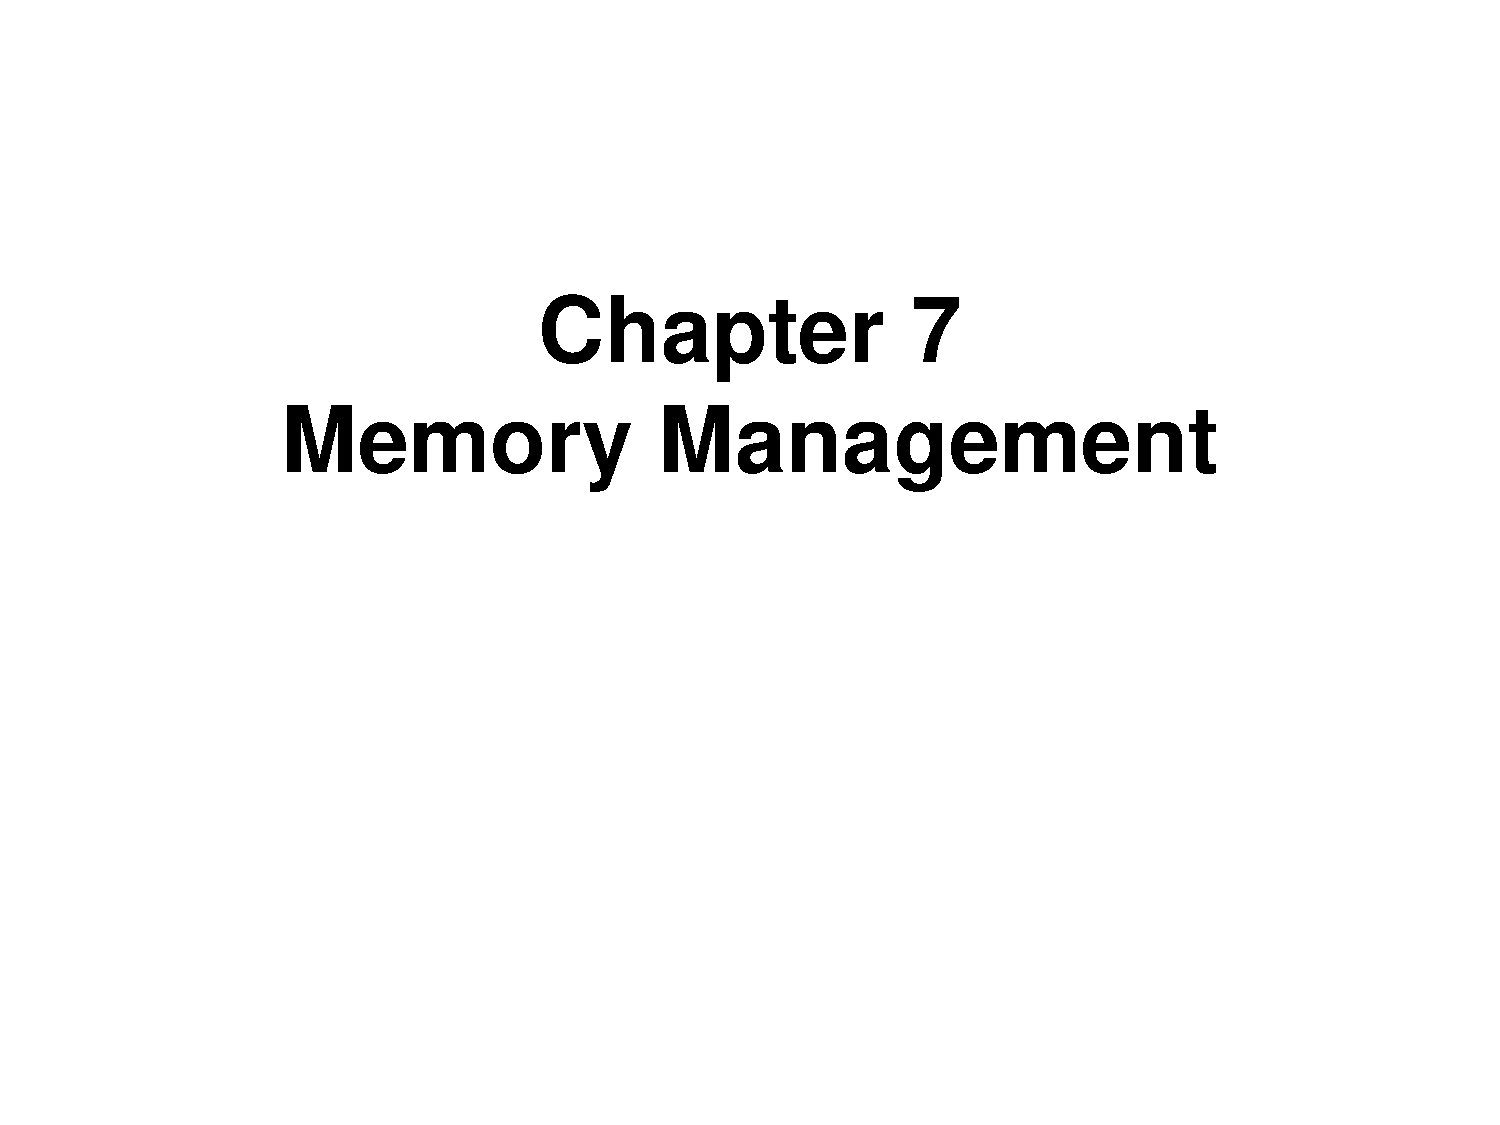
\includepdf[page=1]{07.pdf}
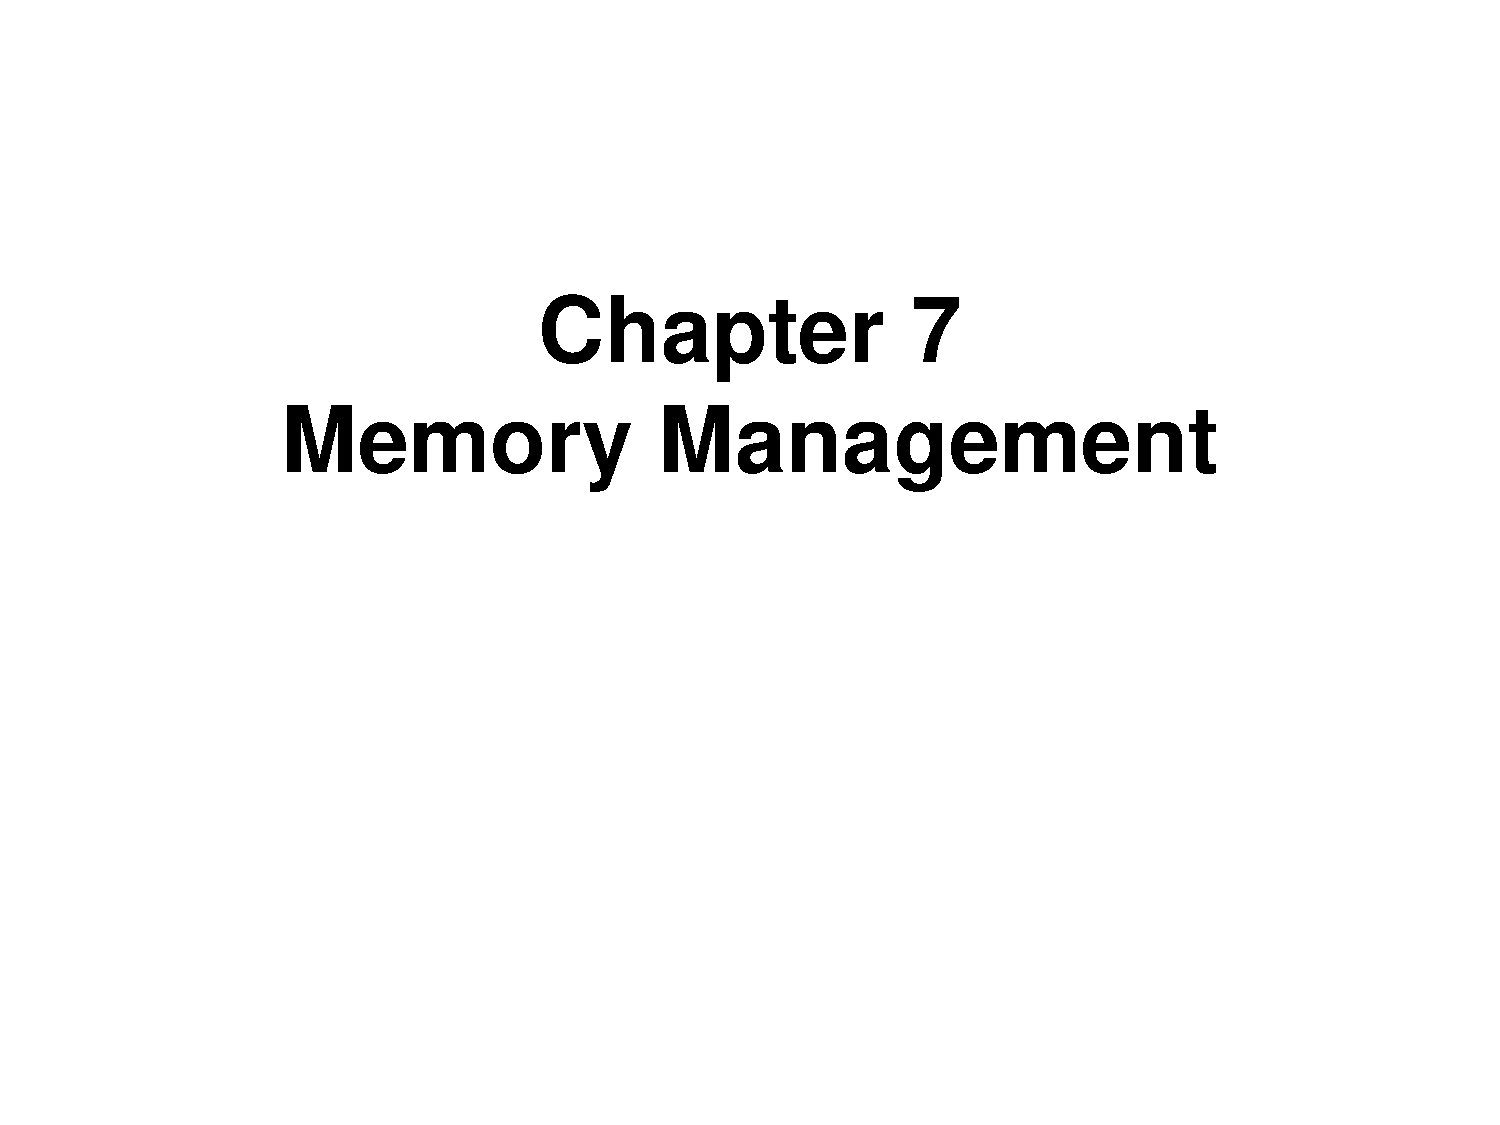
\includepdf[page=2]{07.pdf}
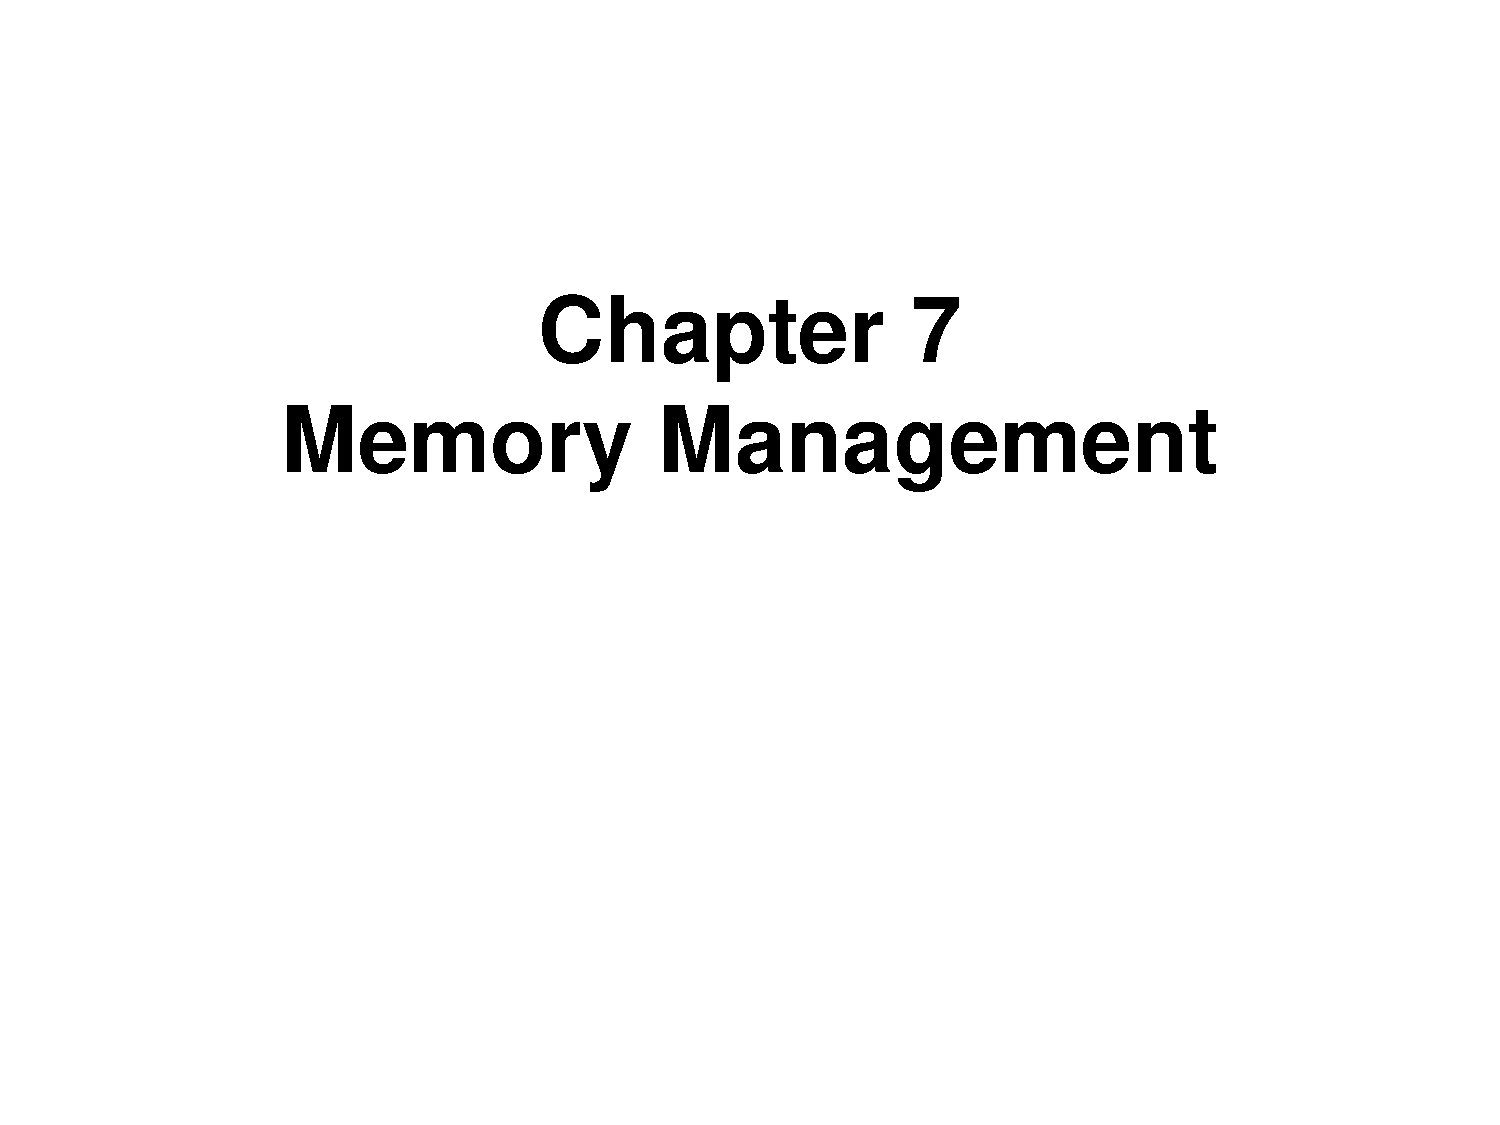
\includepdf[page=3]{07.pdf}
We need to allow the process to shift around in main memory, so when we refer to a global variable in the process things get wonky because the address of the global variable gets mucked when we move things.
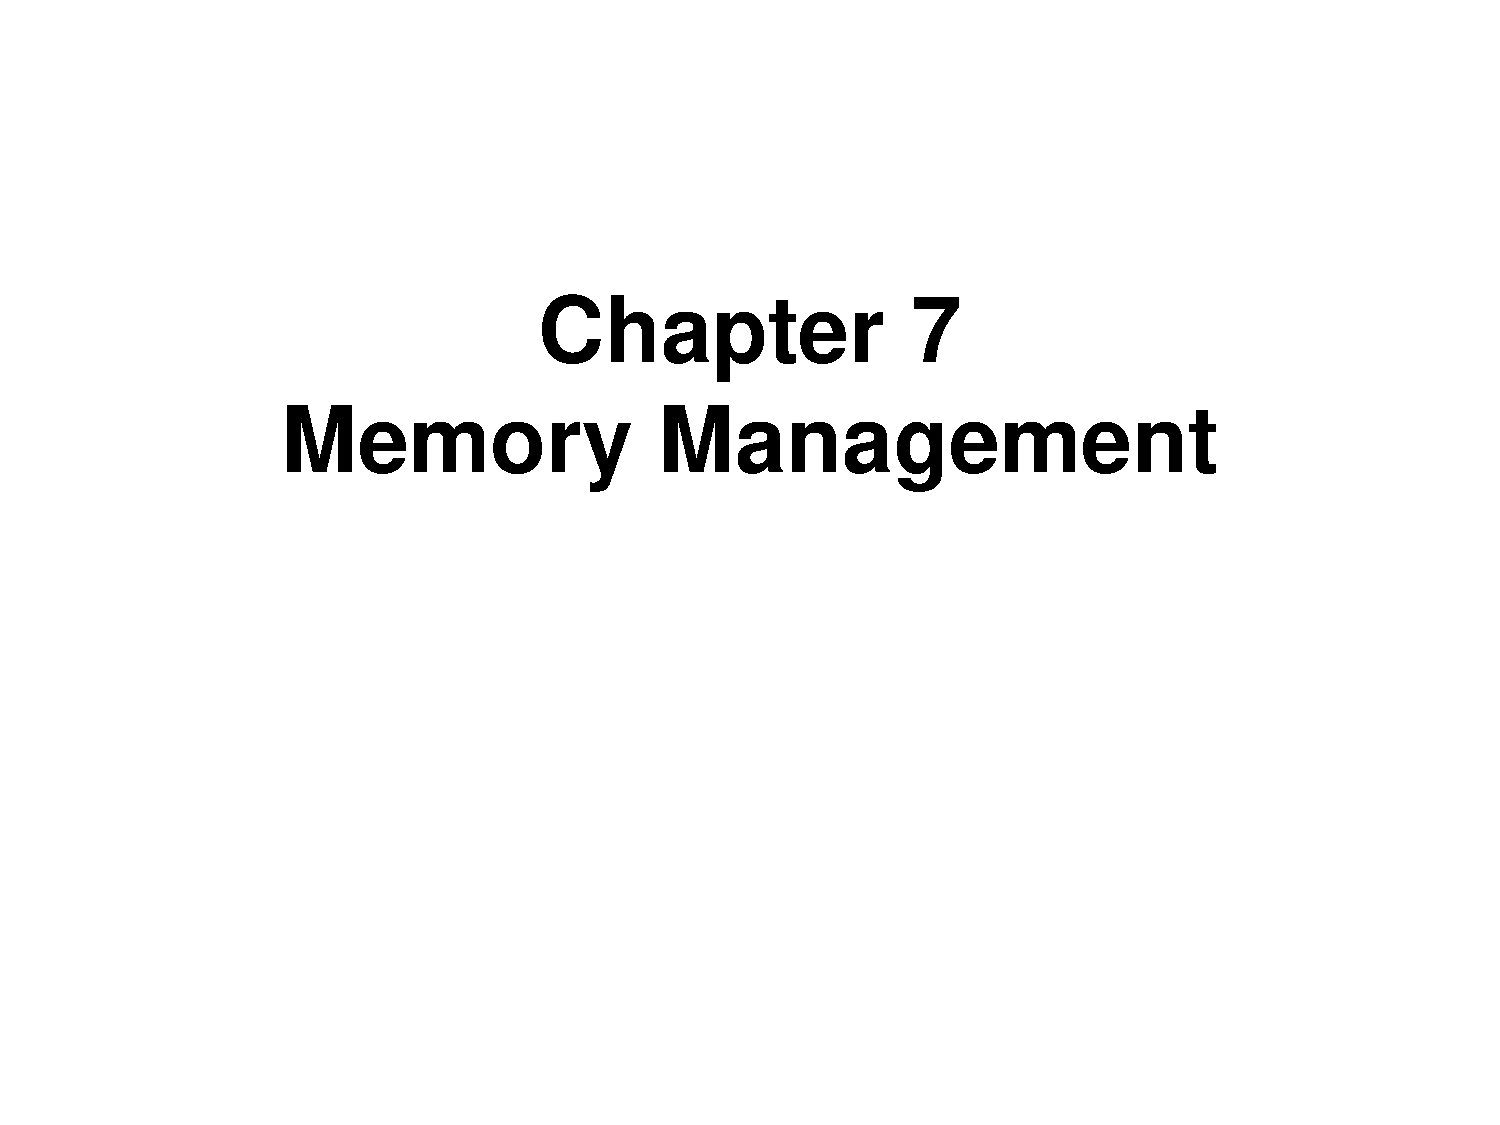
\includepdf[page=4]{07.pdf}
Here is an example of references.
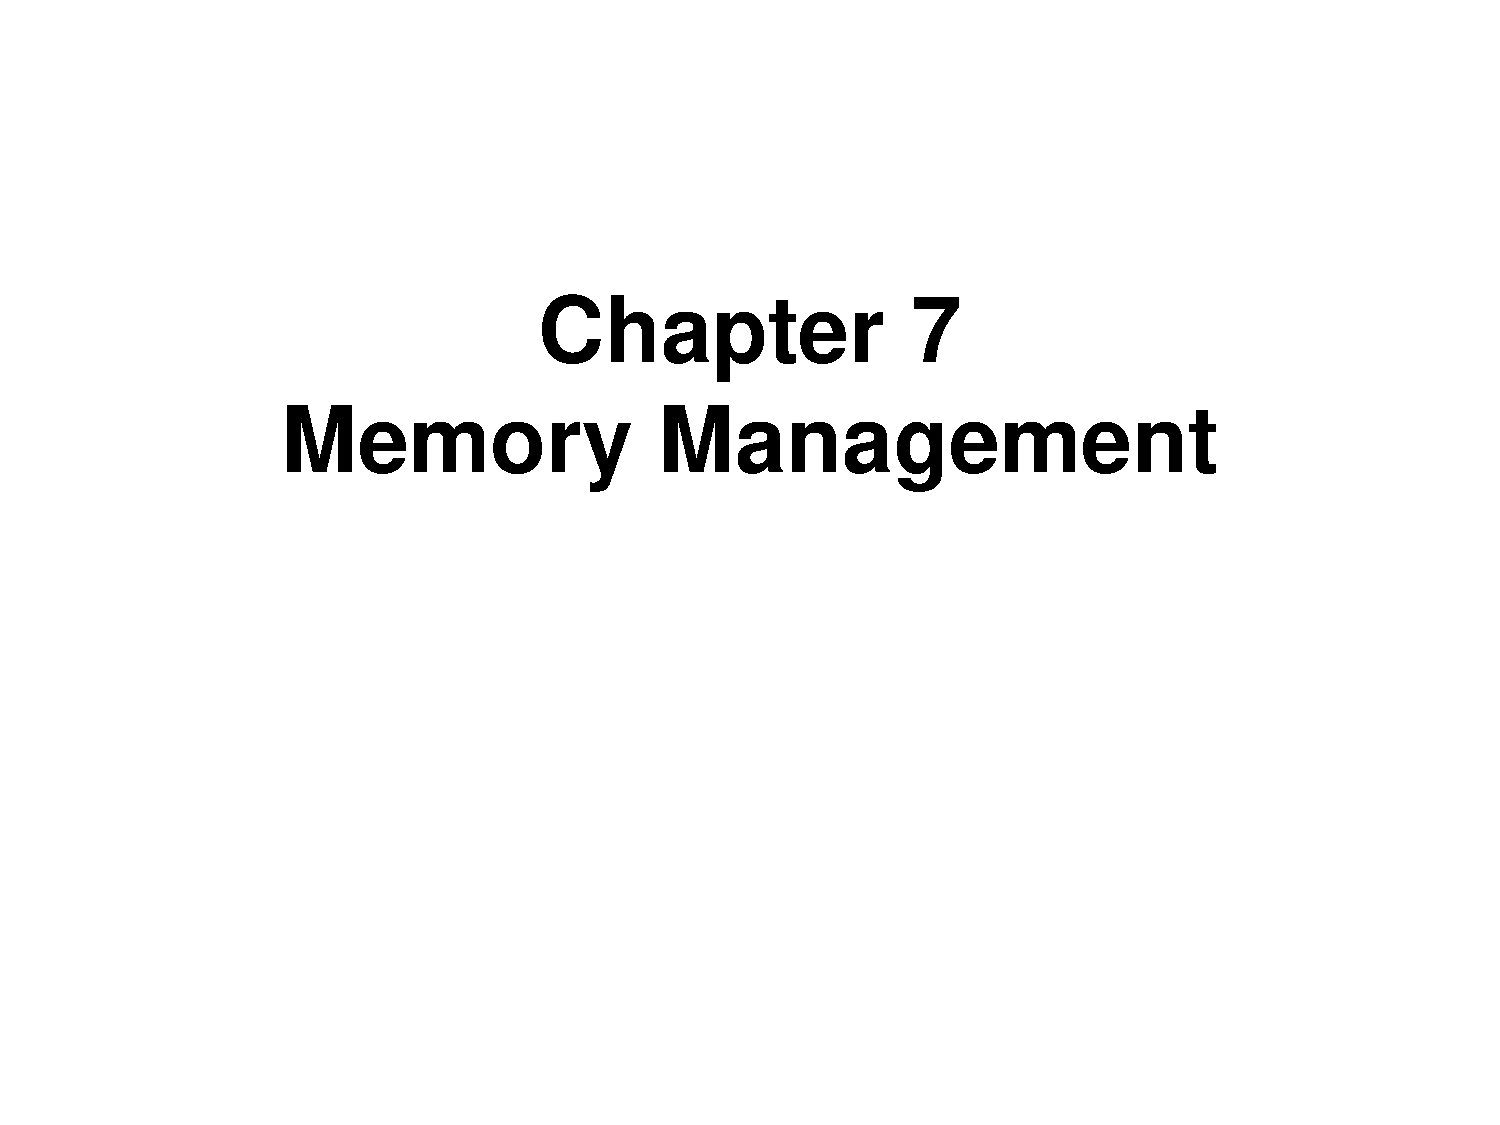
\includepdf[page=5]{07.pdf}
Requirement 1: how do we implement relocation?

Requirement 2: how do we implement protection?\\
We want to make sure that all memory references a process makes is within its owned data and catch when it tries to access memory it doesnt own in main memory.
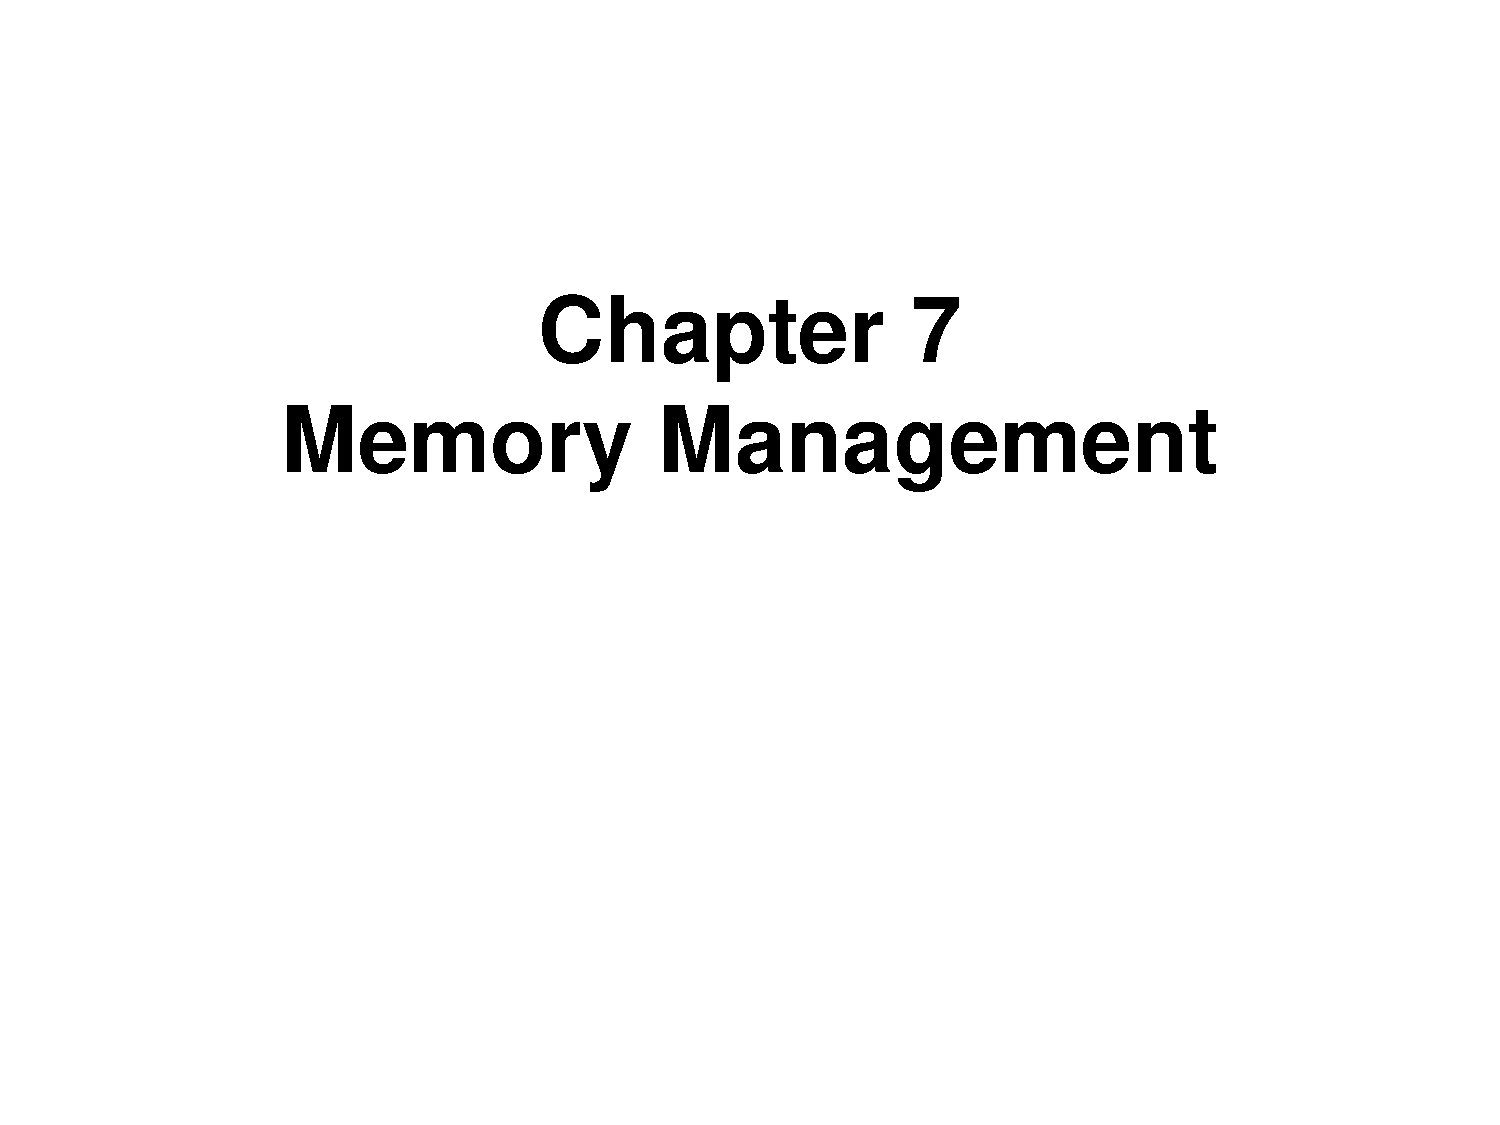
\includepdf[page=6]{07.pdf}
Requirement 3: how do we implement sharing?\\
We need to allocate a shared peice of memory (shared by process A and B)
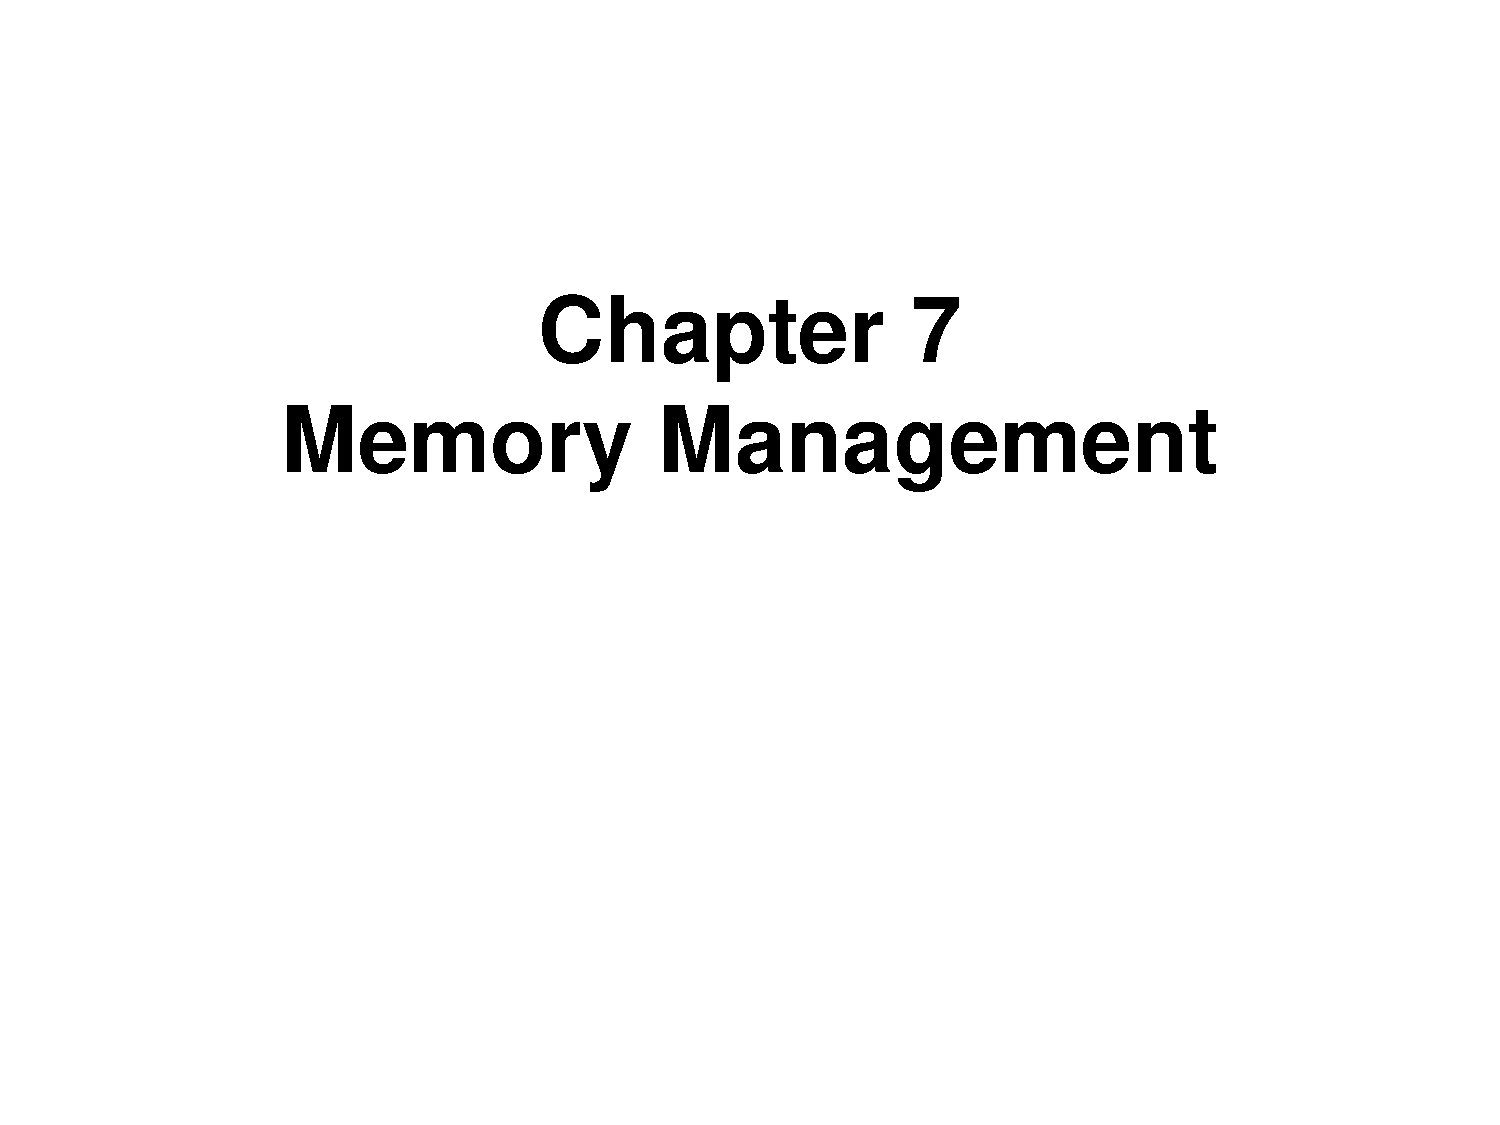
\includepdf[page=7]{07.pdf}
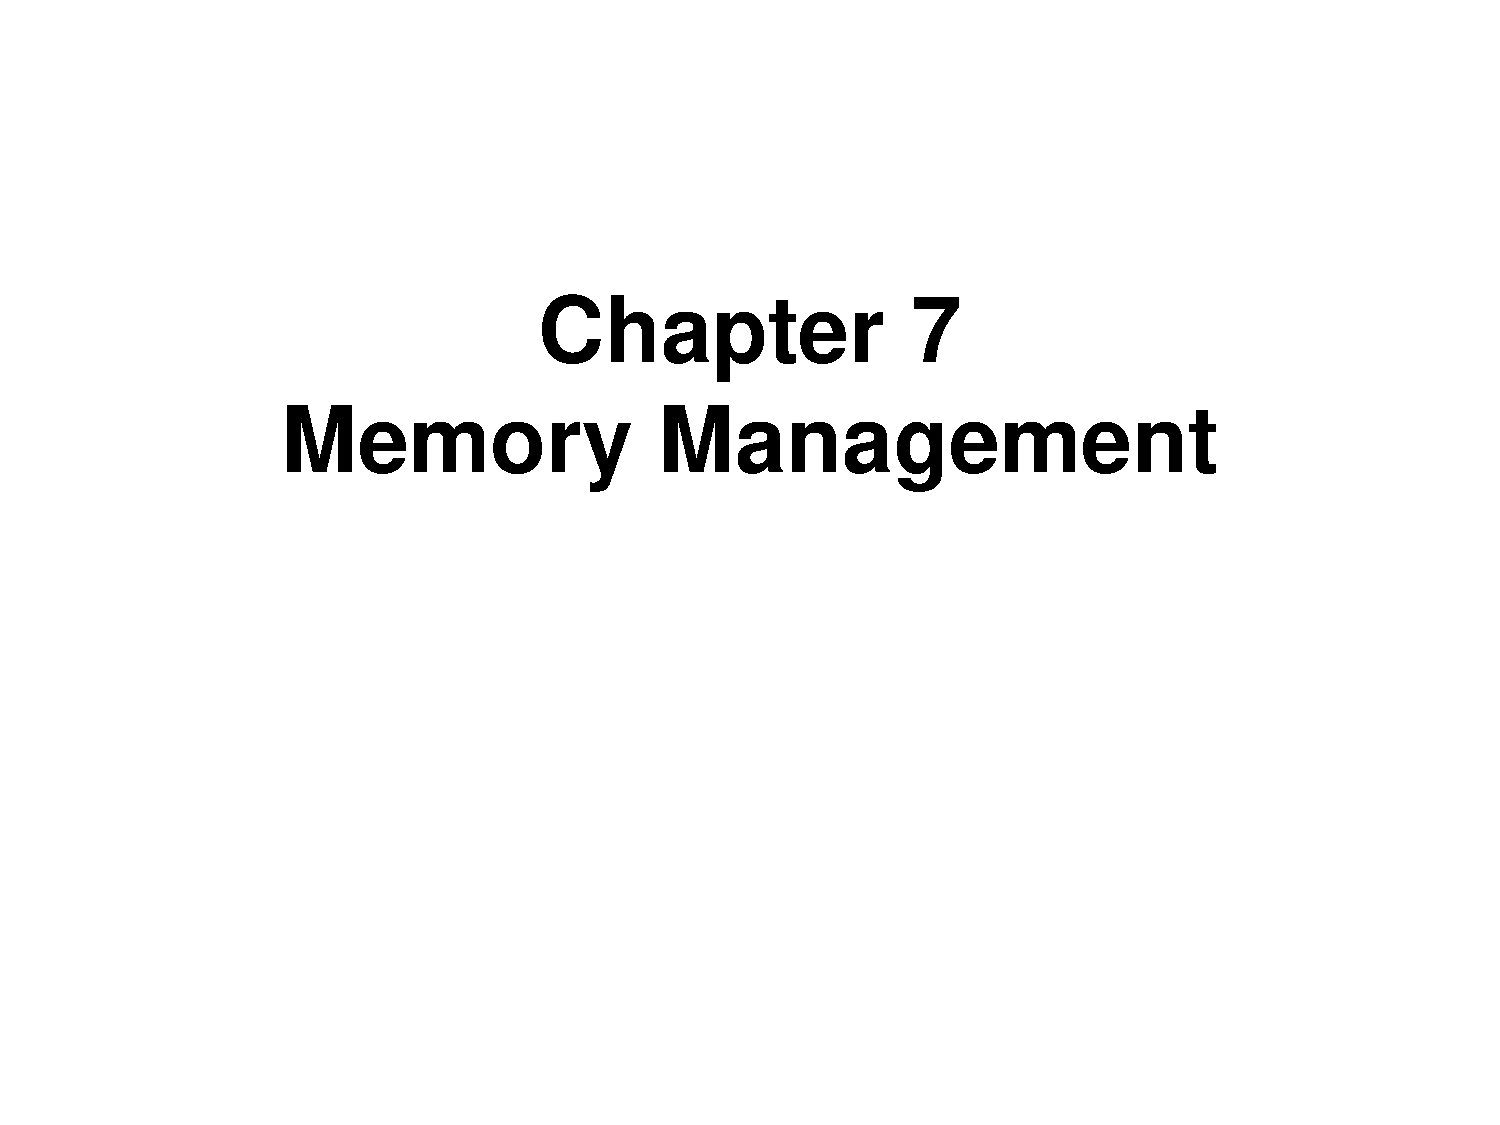
\includepdf[page=8]{07.pdf}
Requrement 5: how do we implement physical organization\\
How do we organize the physical space so that we can have enough for each program without knowing what they need at the start.
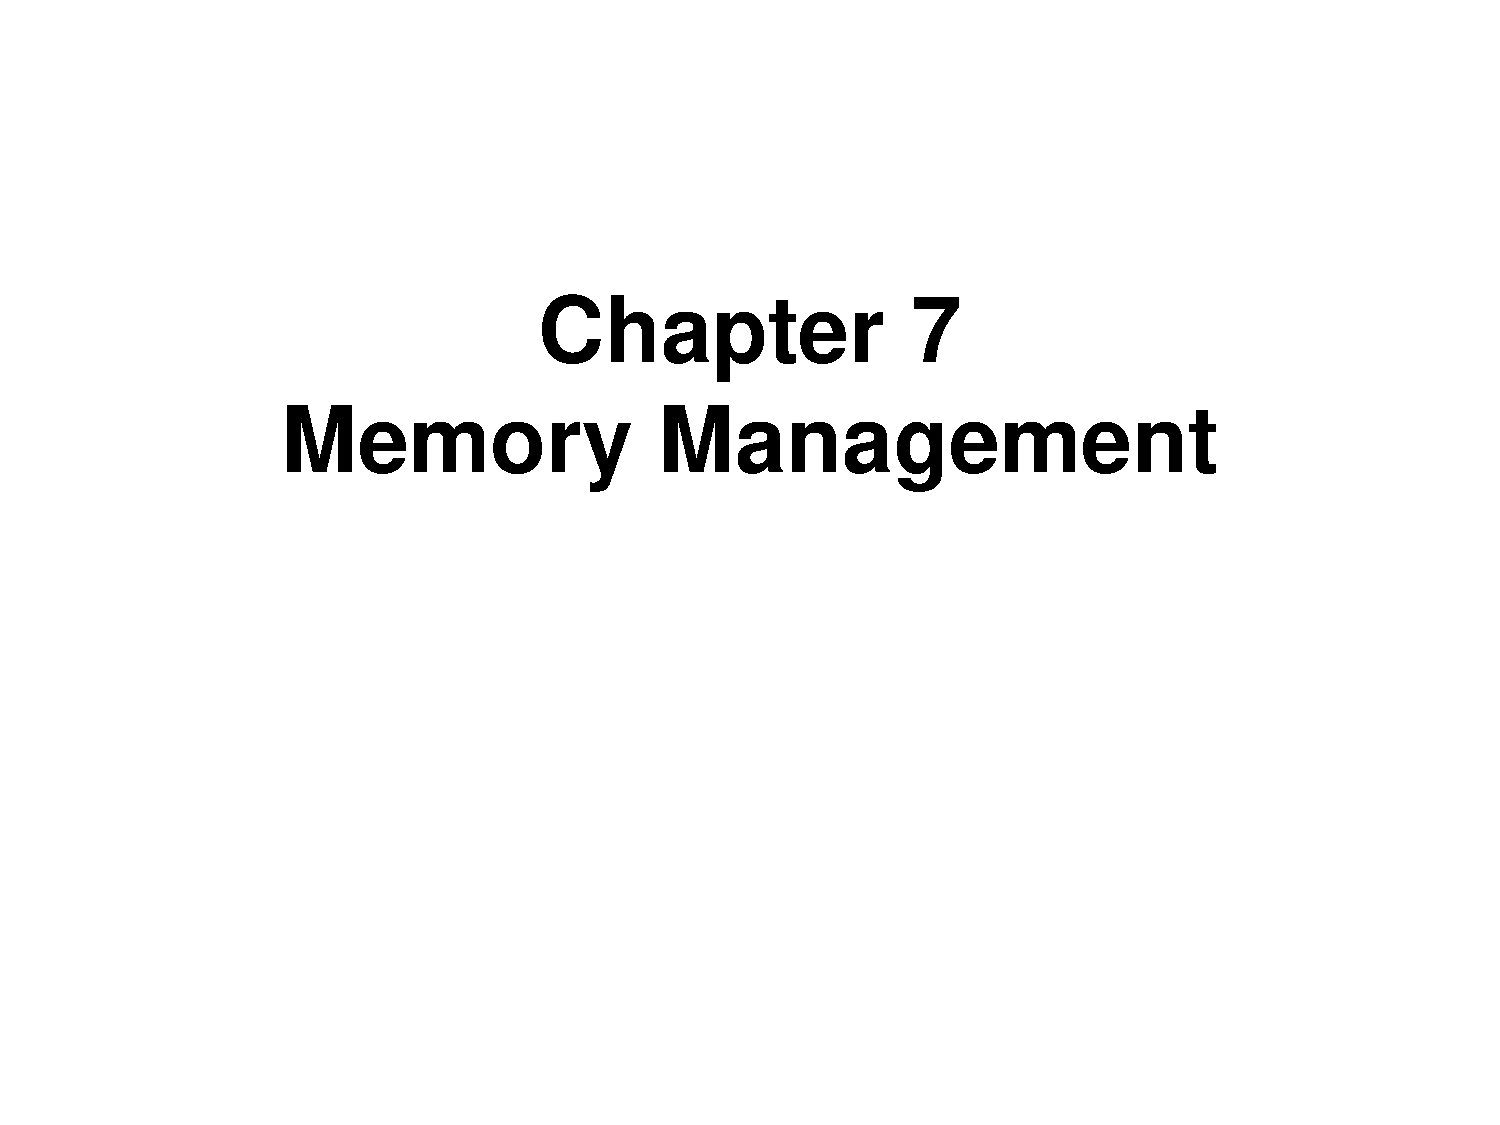
\includepdf[page=9]{07.pdf}
One method to implement physical organization is to have a fixed chunk size of memory. When a process is loaded it is stored in one chunk (programs are limited by chunk size since they cannot span multiple chunks). Here the programmer doesnt need to know what the total size of memory is but is instead constrained in the size of their program. It is also inefficient because process that is smaller than the chunk has unused space resulting in fragmented memory. Internal fragmentation only occurs here when the process image is smaller than the partition size.
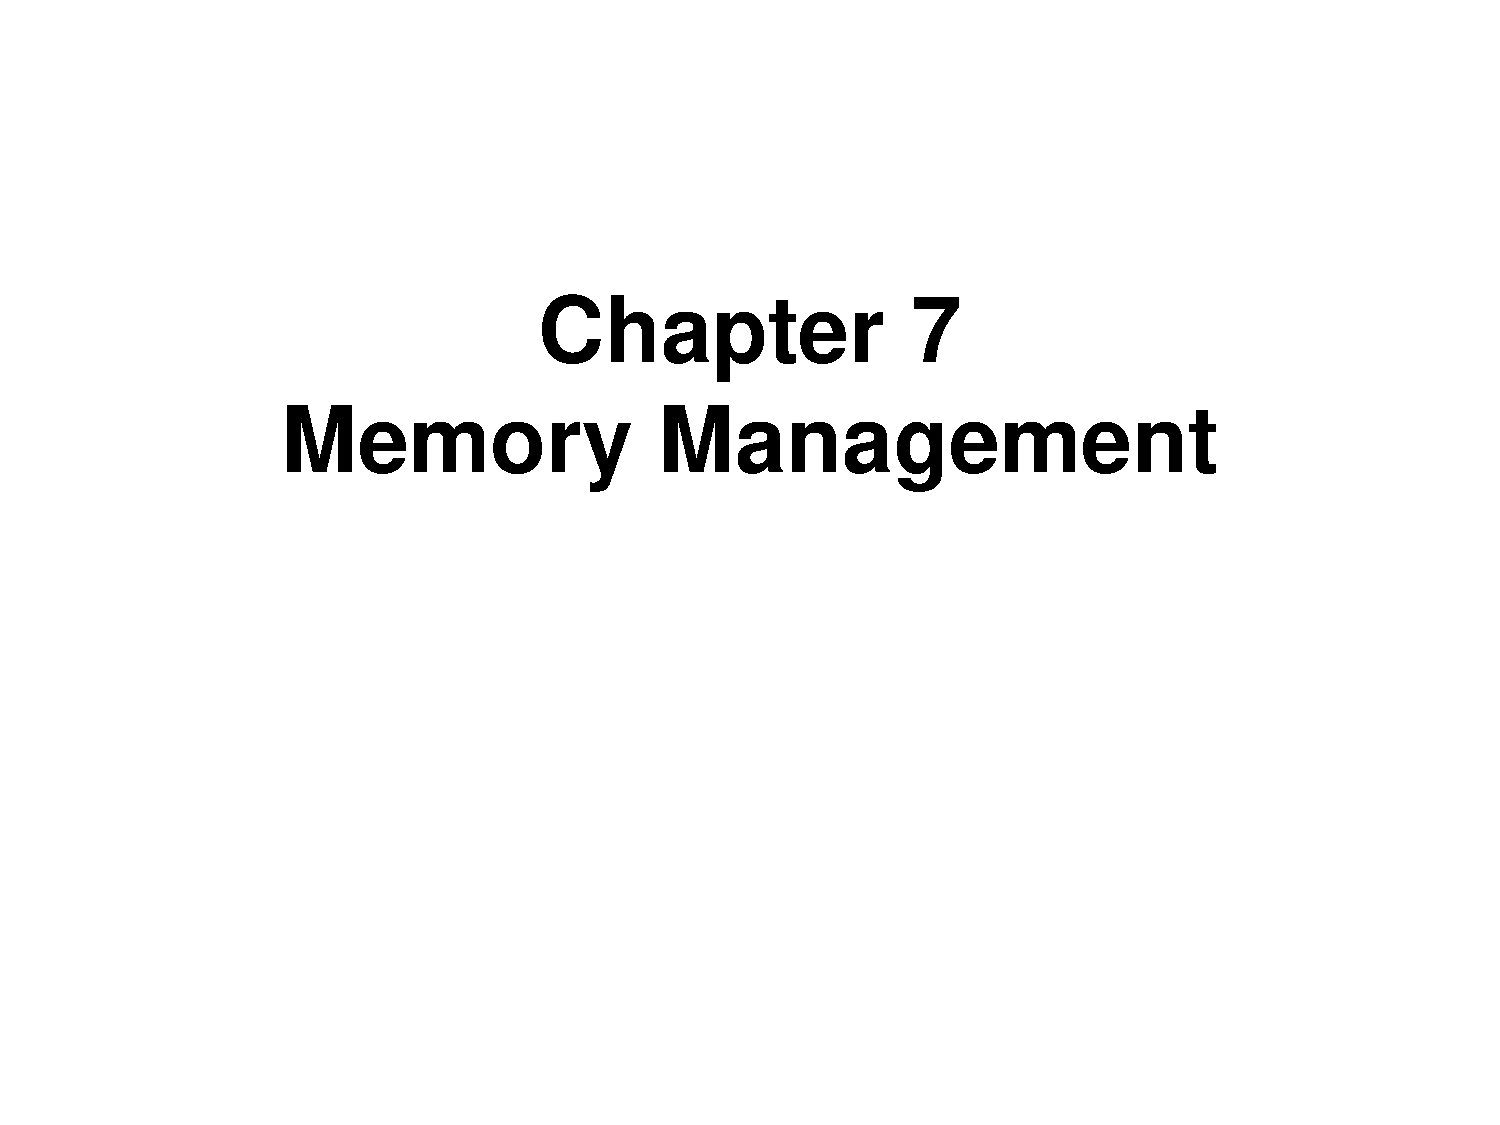
\includepdf[page=10]{07.pdf}
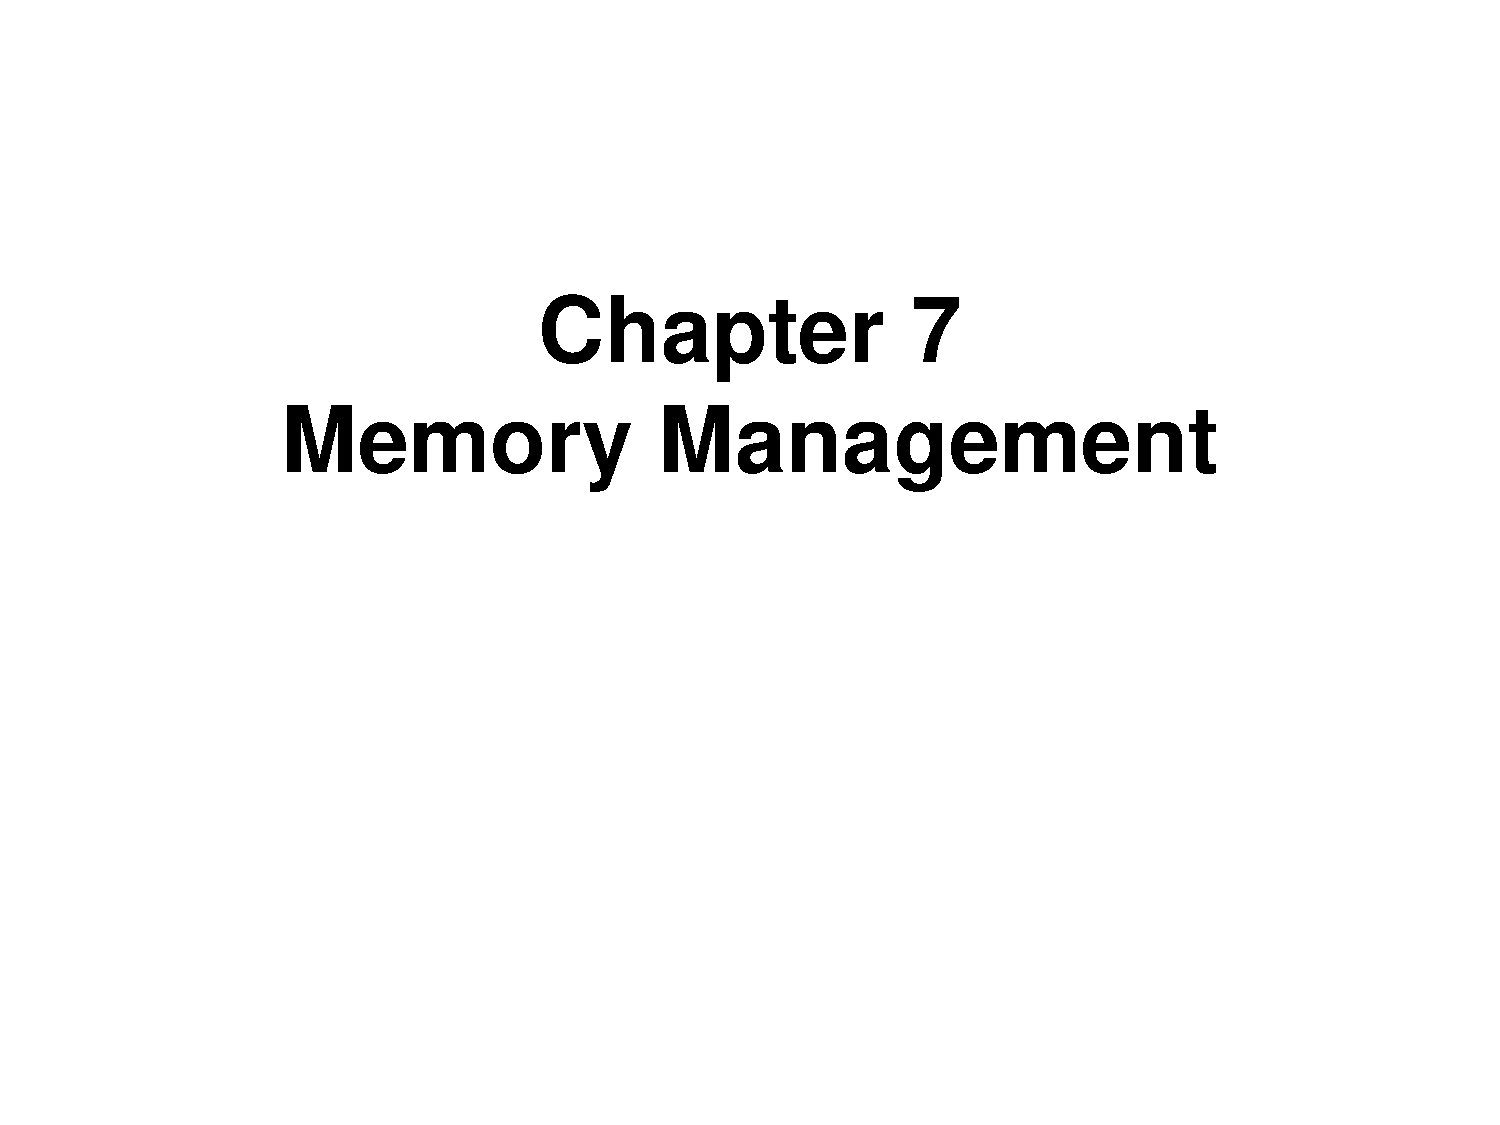
\includepdf[page=11]{07.pdf}
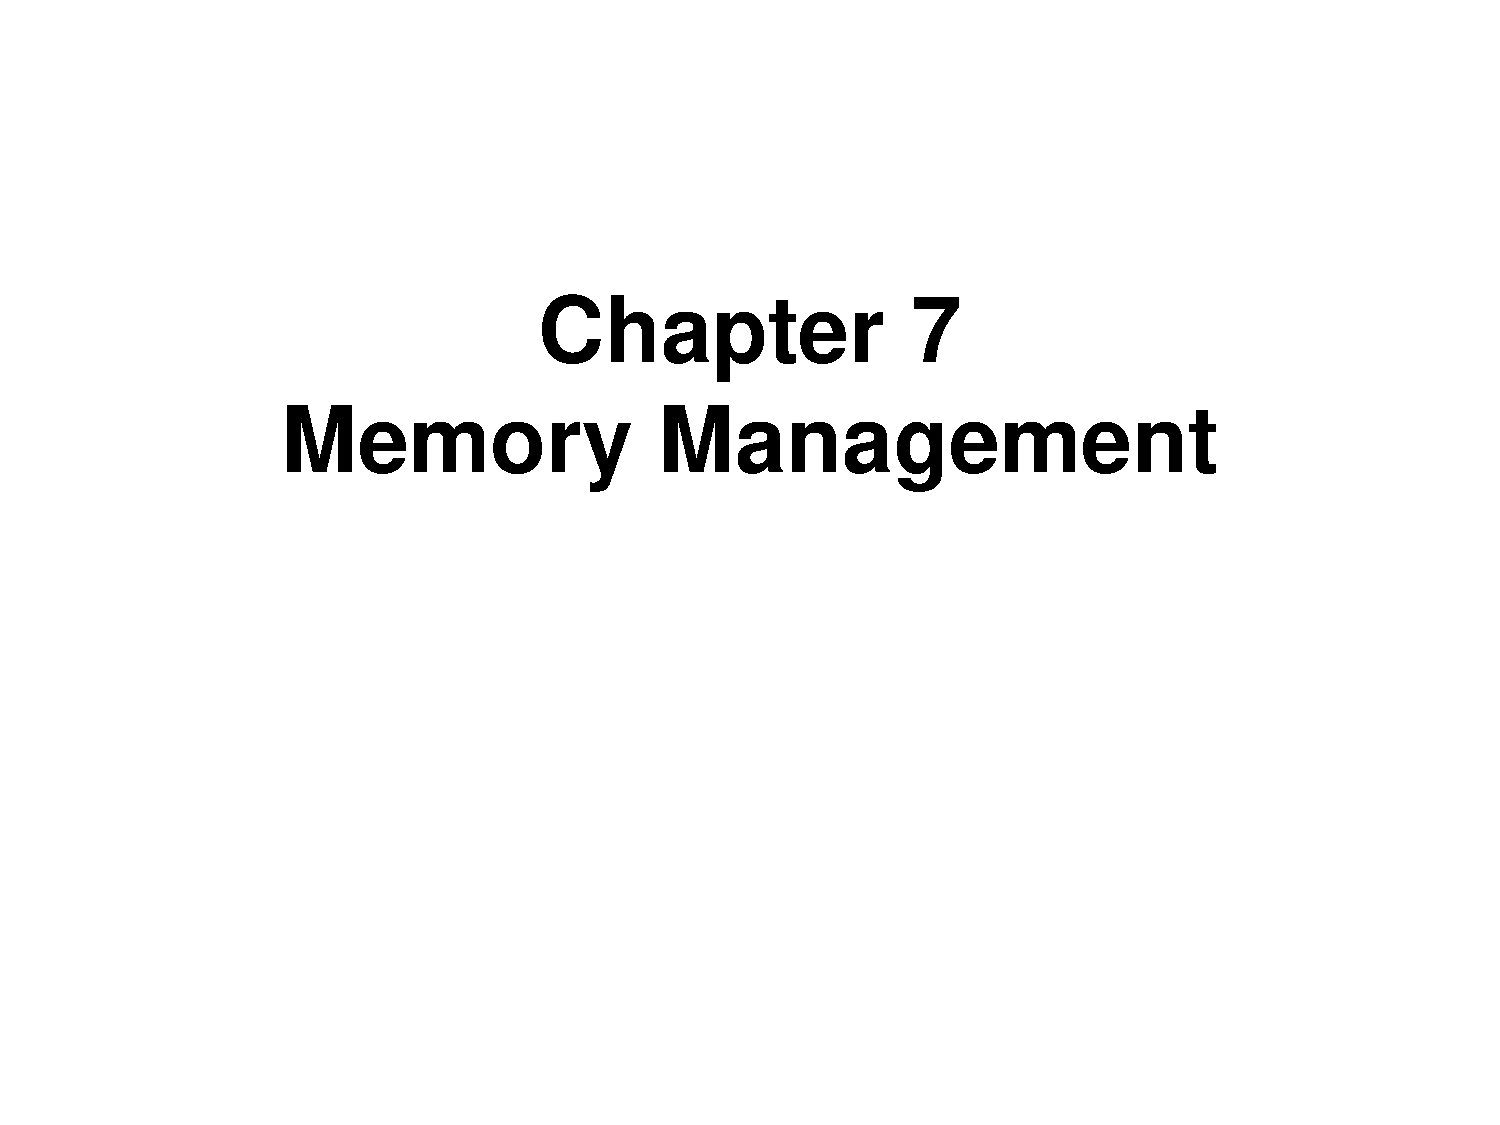
\includepdf[page=12]{07.pdf}
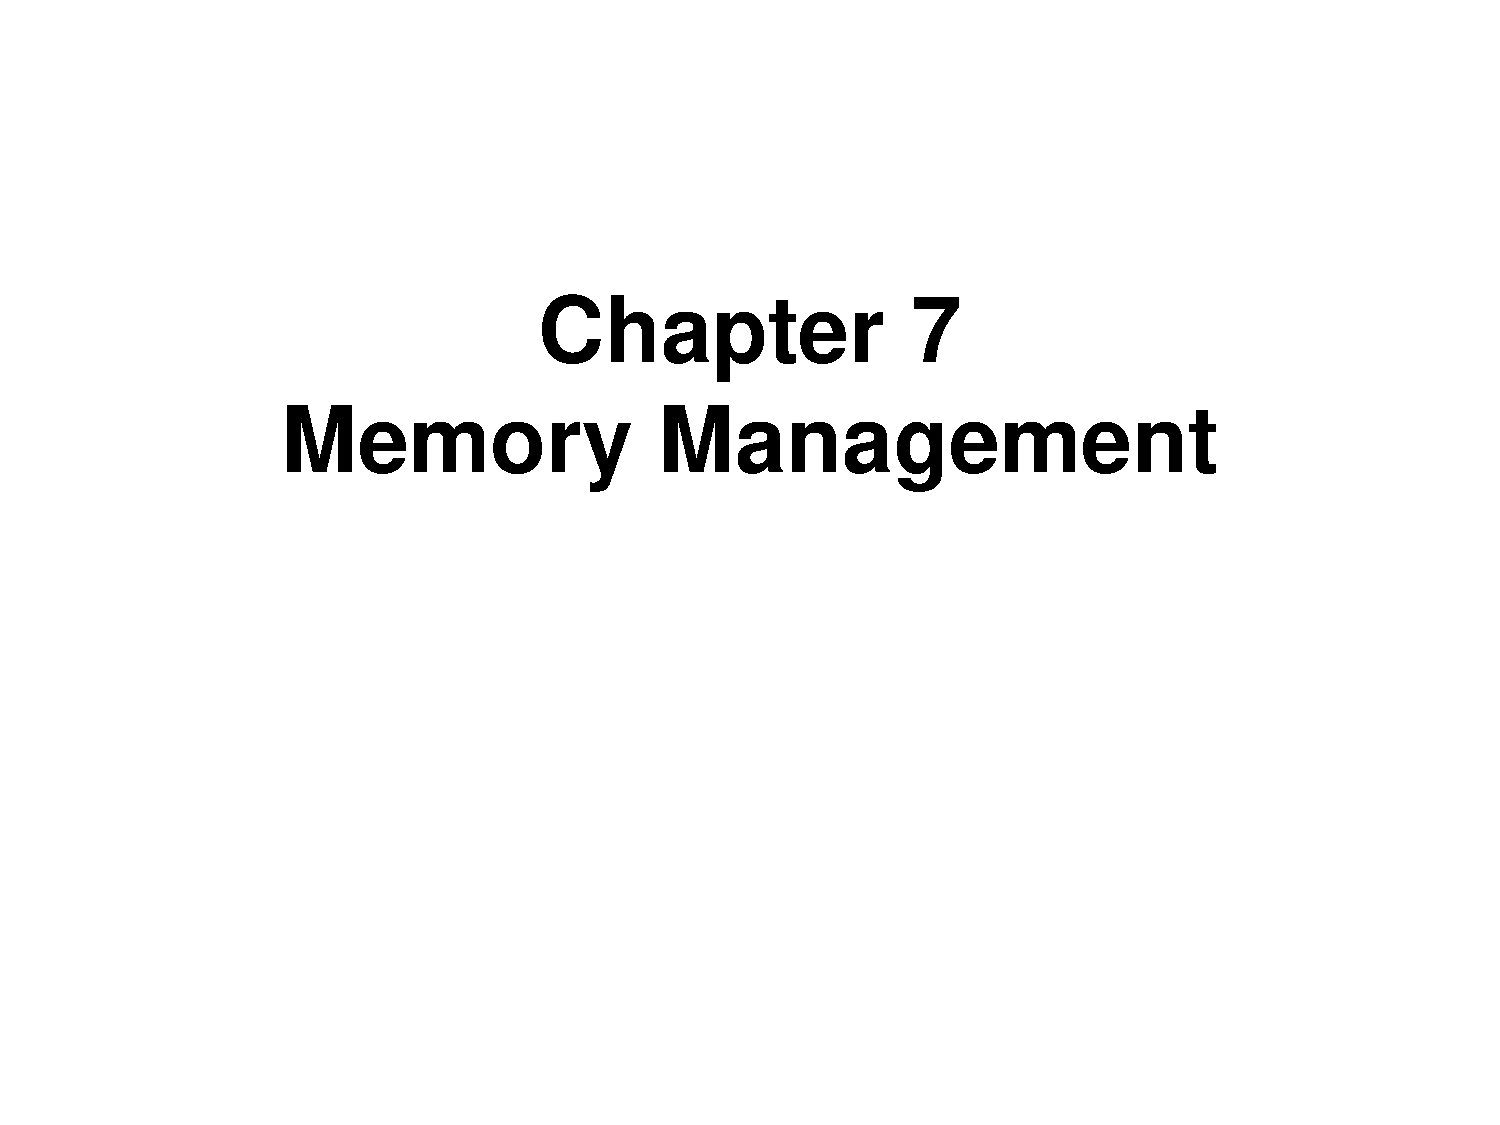
\includepdf[page=13]{07.pdf}
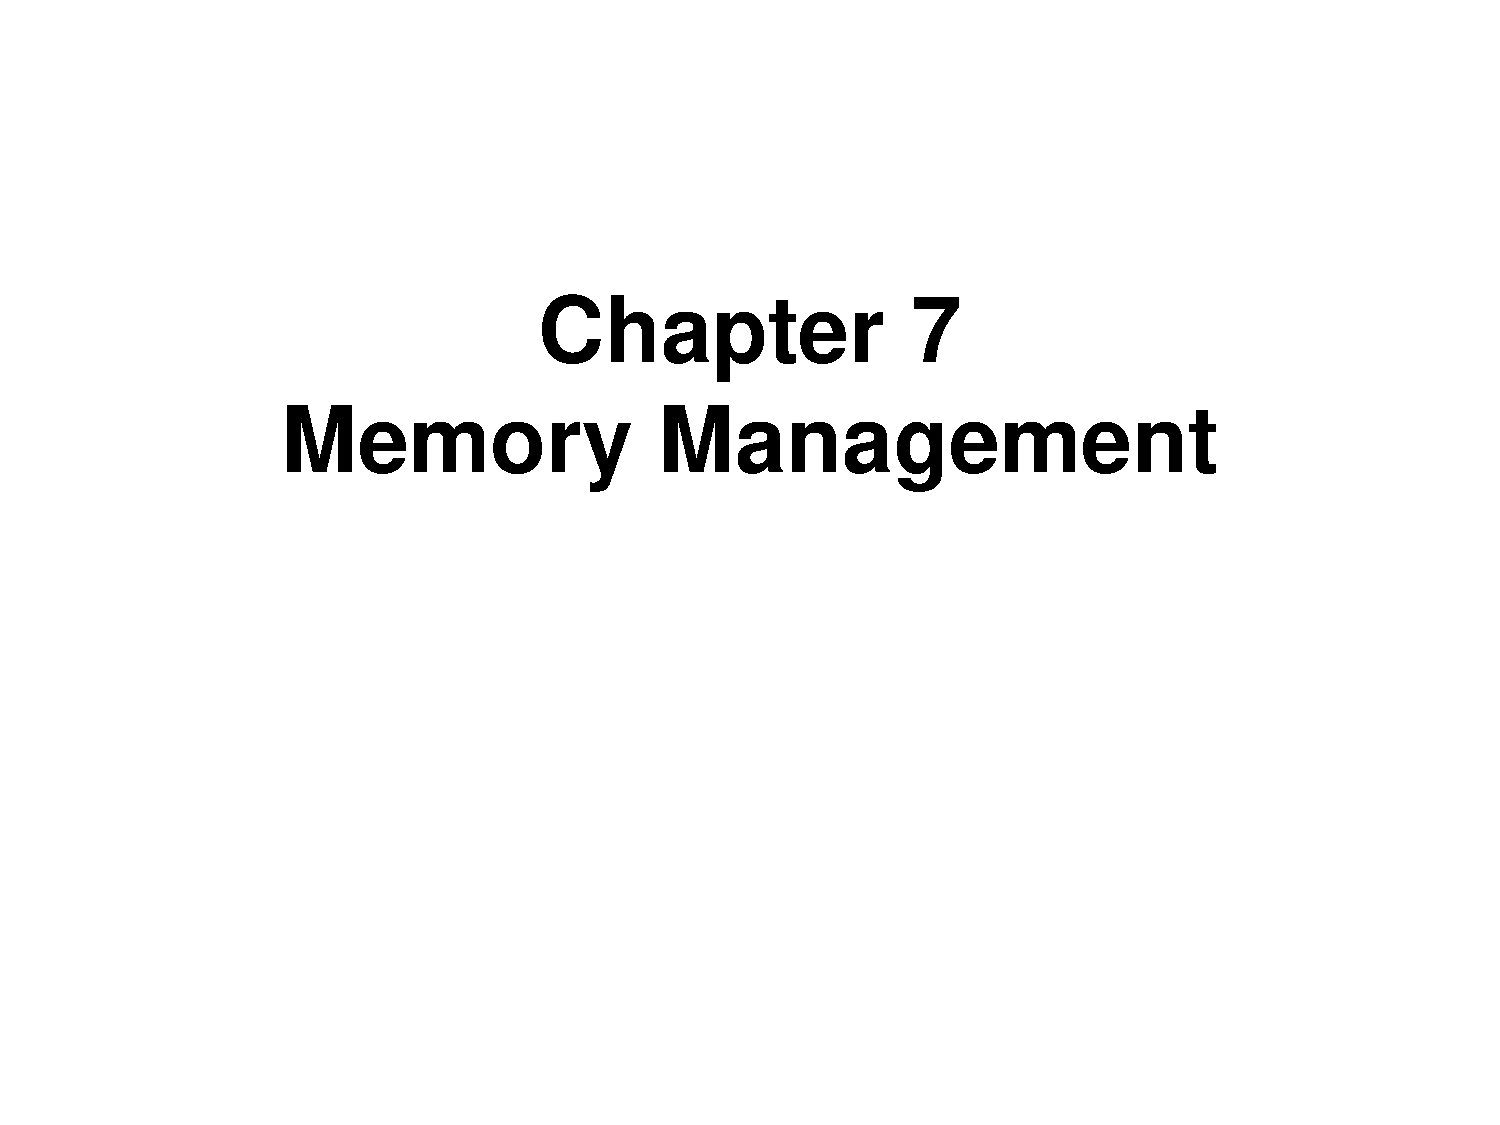
\includepdf[page=14]{07.pdf}
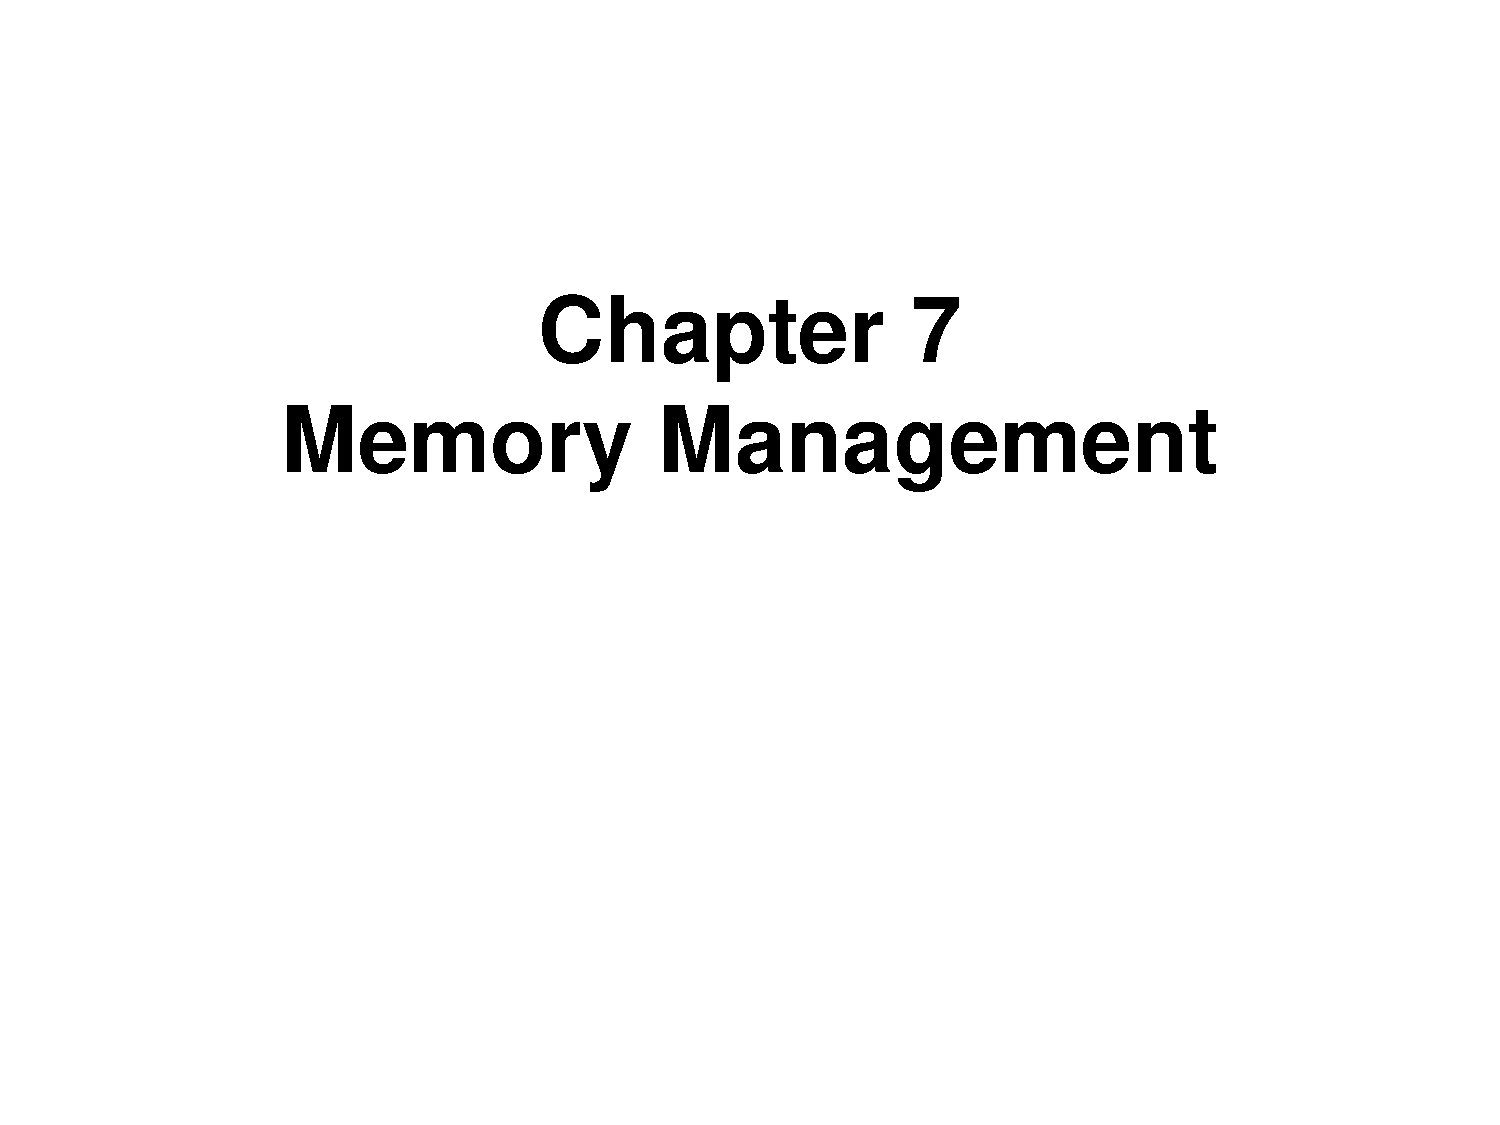
\includepdf[page=15]{07.pdf}
This is one step up. Instead of fixing the size of the partion at boot up we expand the allocated size to exactly what the process needs. We can still get fragmentation, but here its called external fragmentation.
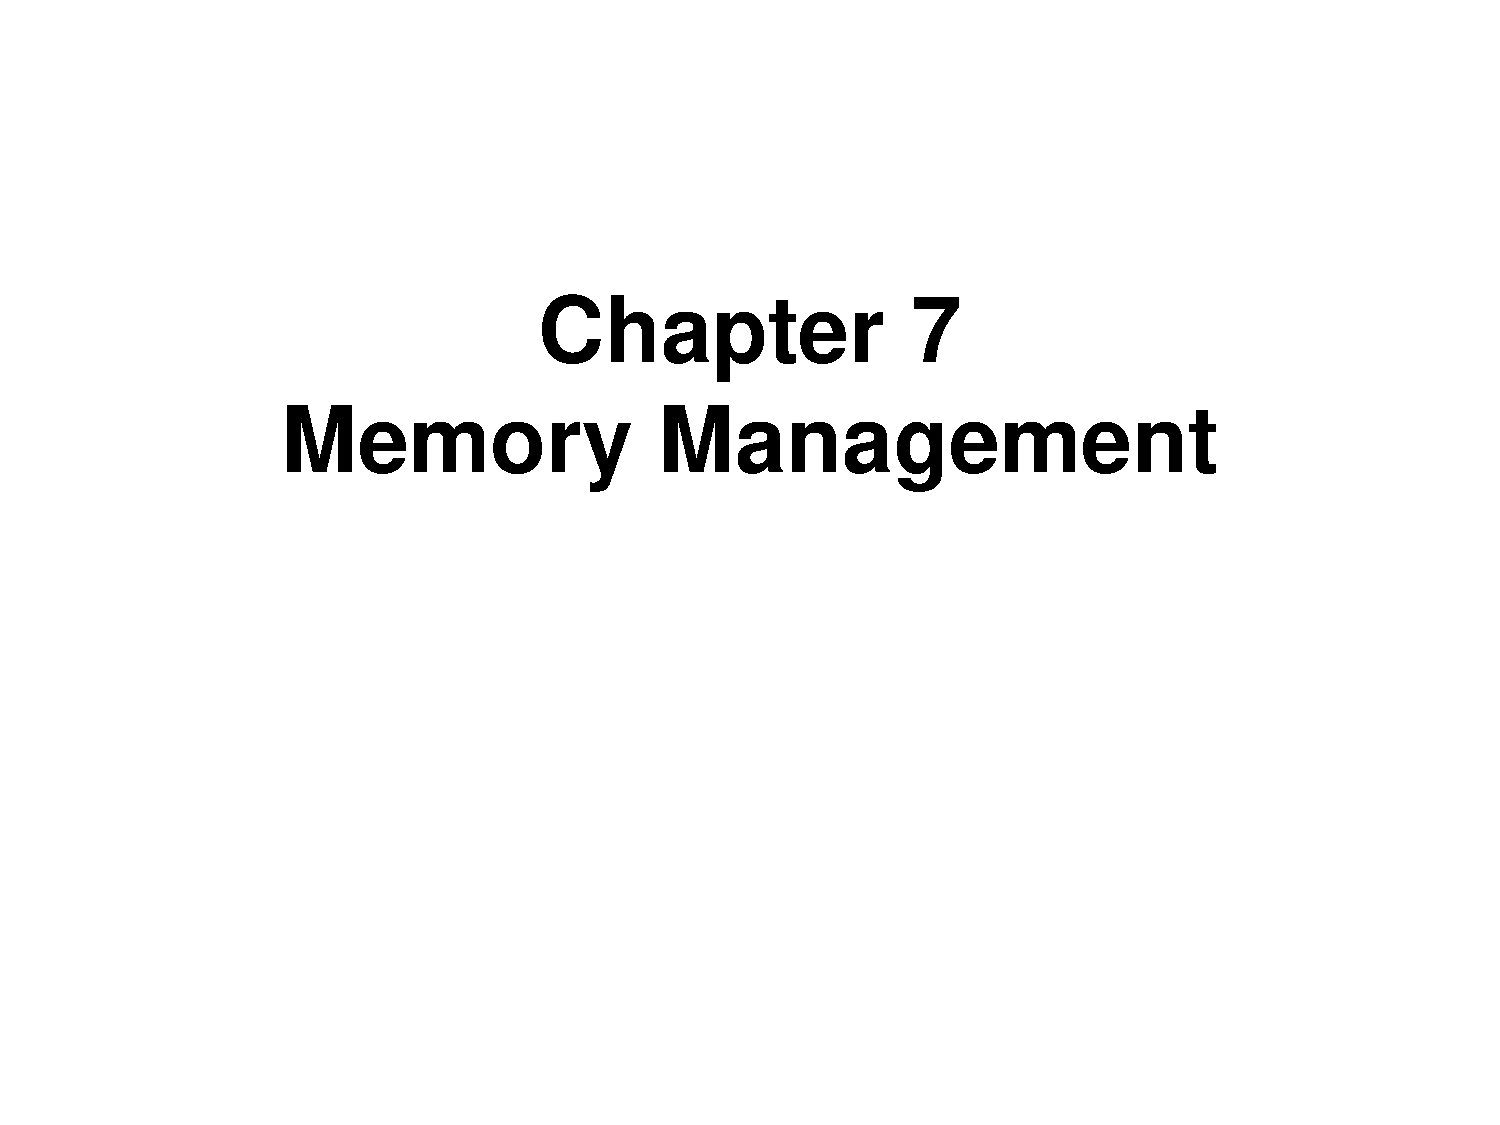
\includepdf[page=16]{07.pdf}
We leave the entire chunk of memory unallocated and when a process is loaded we give it exactly the size of its program image.
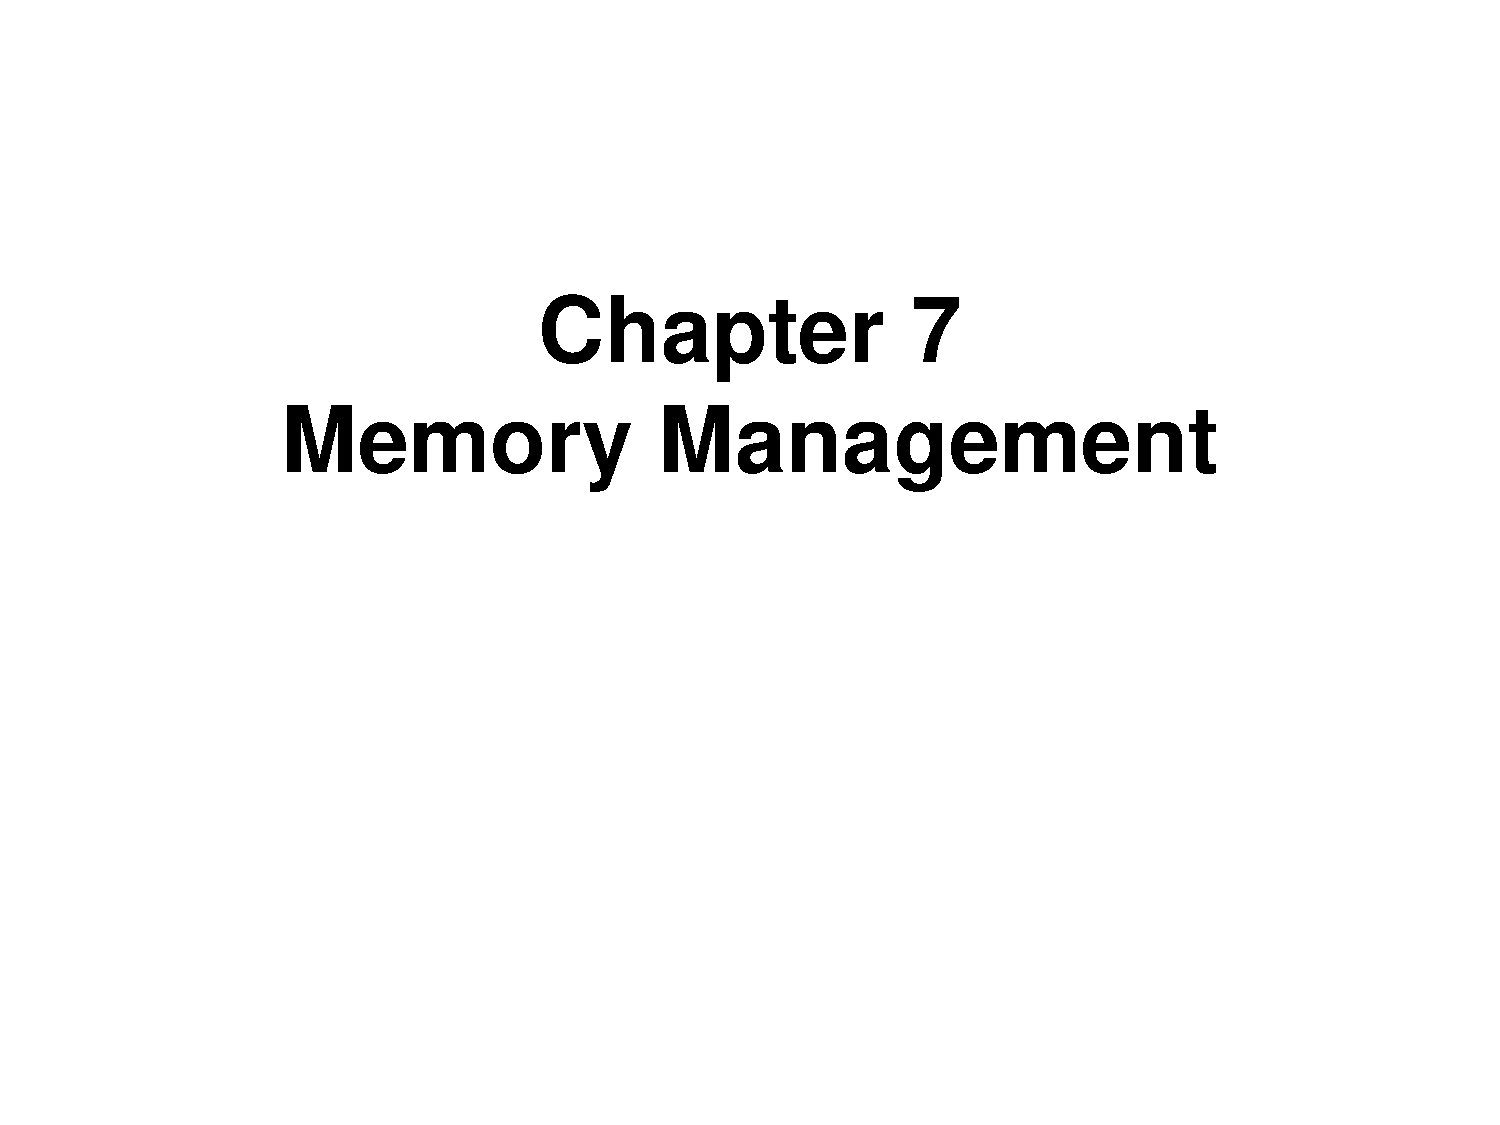
\includepdf[page=17]{07.pdf}
Here we see holes appearing when we swap processes in and out.
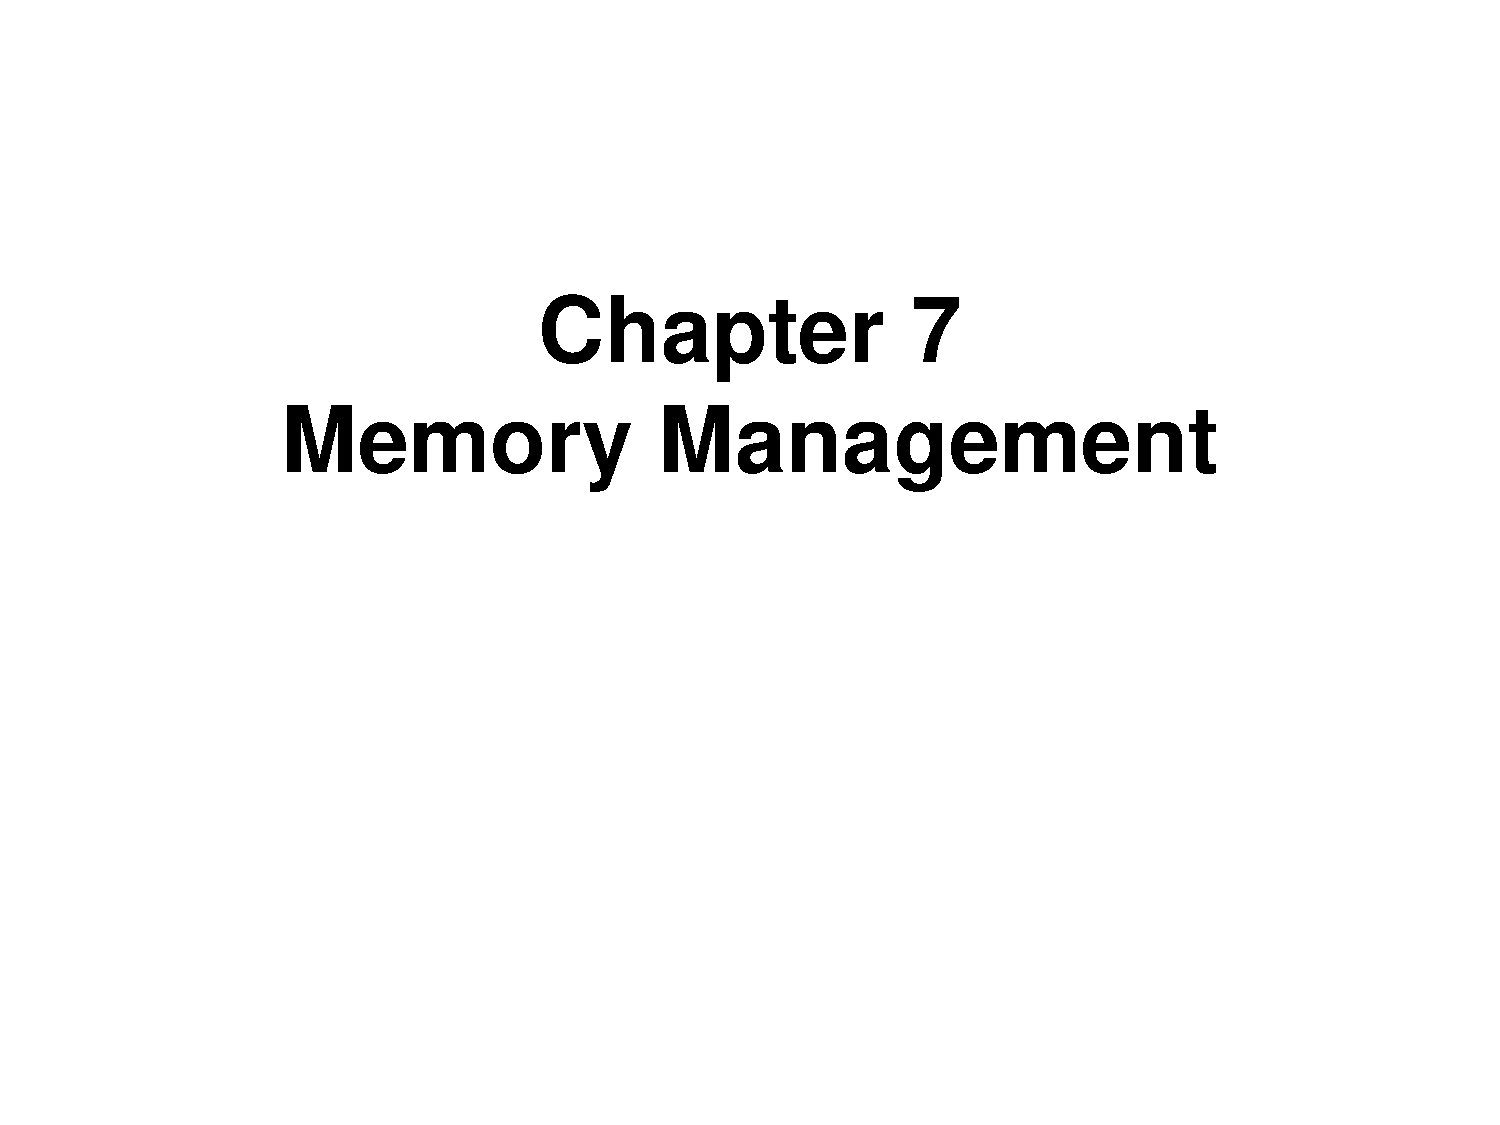
\includepdf[page=18]{07.pdf}
Look at available memory blocks and pick the block that is closest to your memory size. Over time this is the worst fragmenter of you memory.
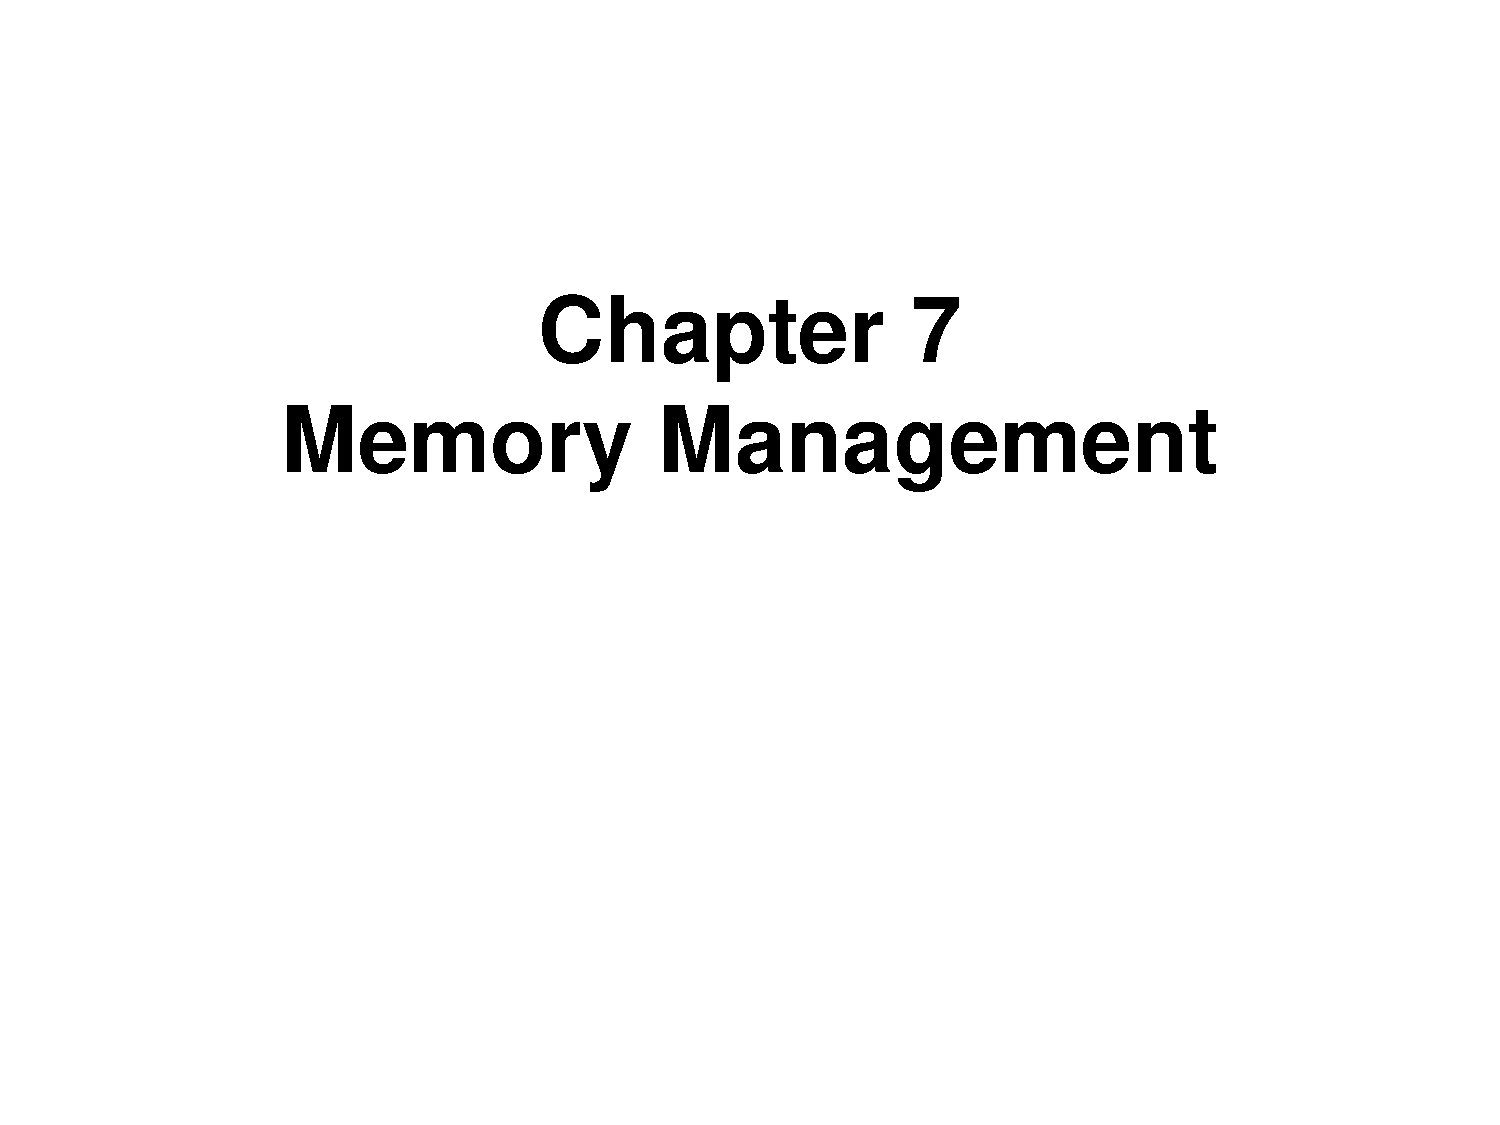
\includepdf[page=19]{07.pdf}
Choses the first block that is large enough for your process. This is the fastest but we get lots of processes at the front of the memory block so scanning takes longer as you go.
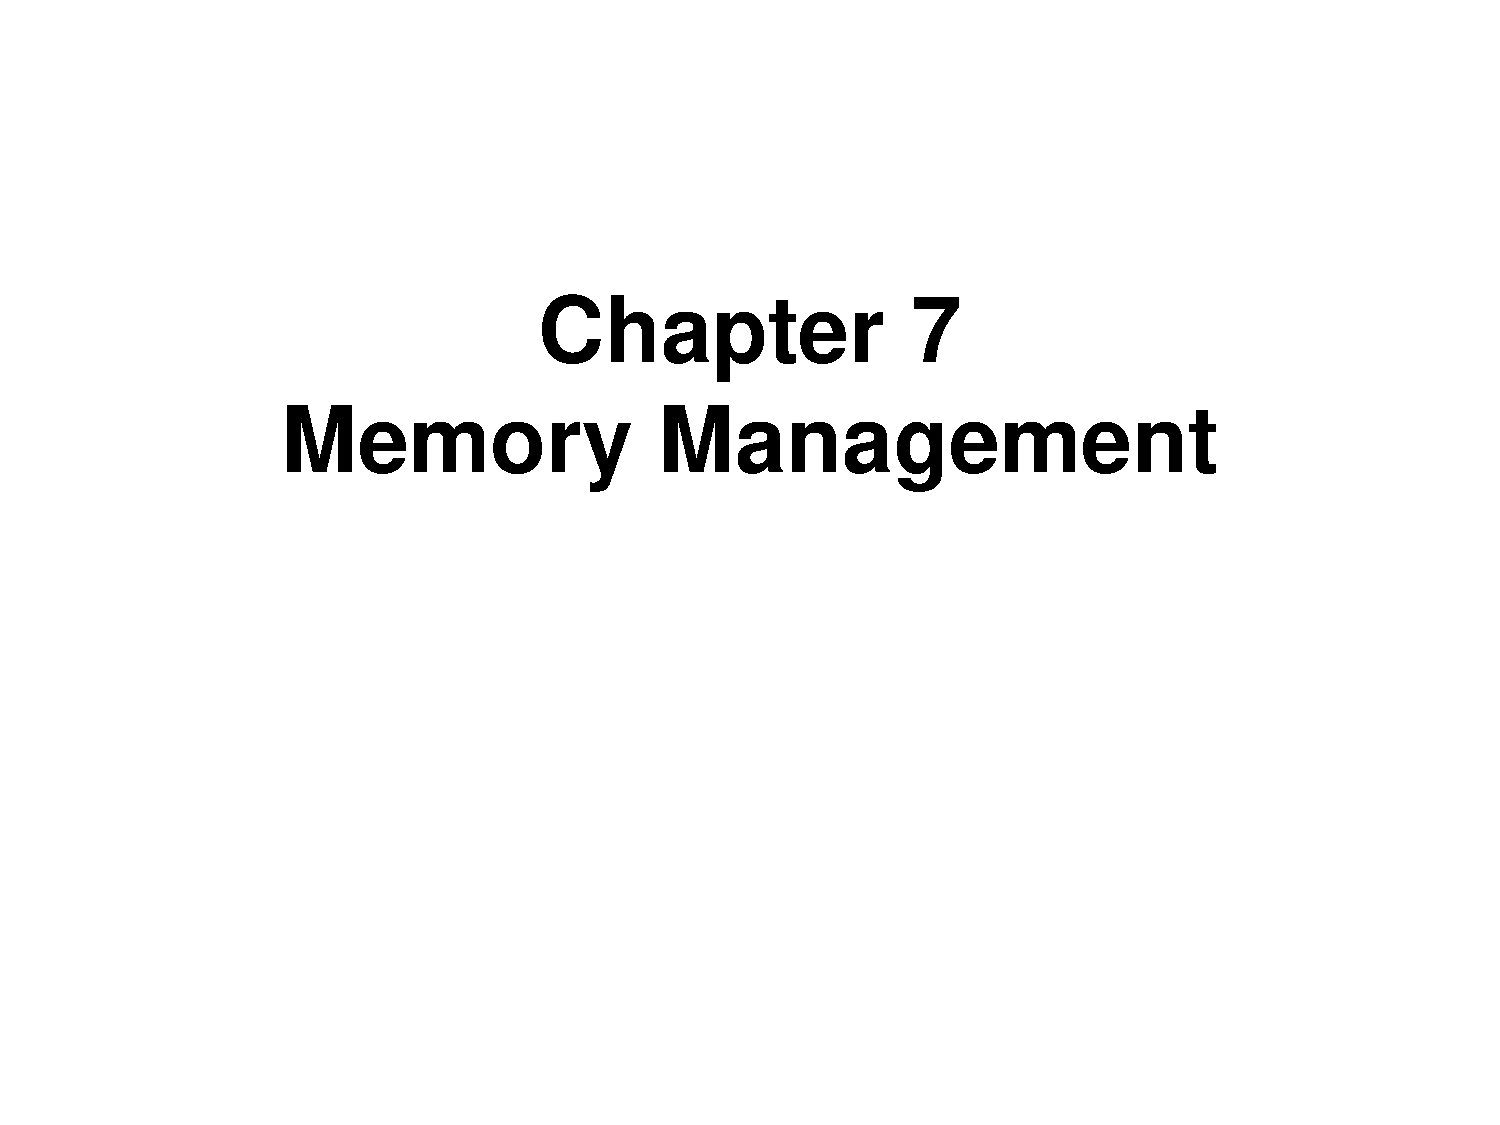
\includepdf[page=20]{07.pdf}
Start allocating space from the last allocated space of memory (think of a linked list ish).
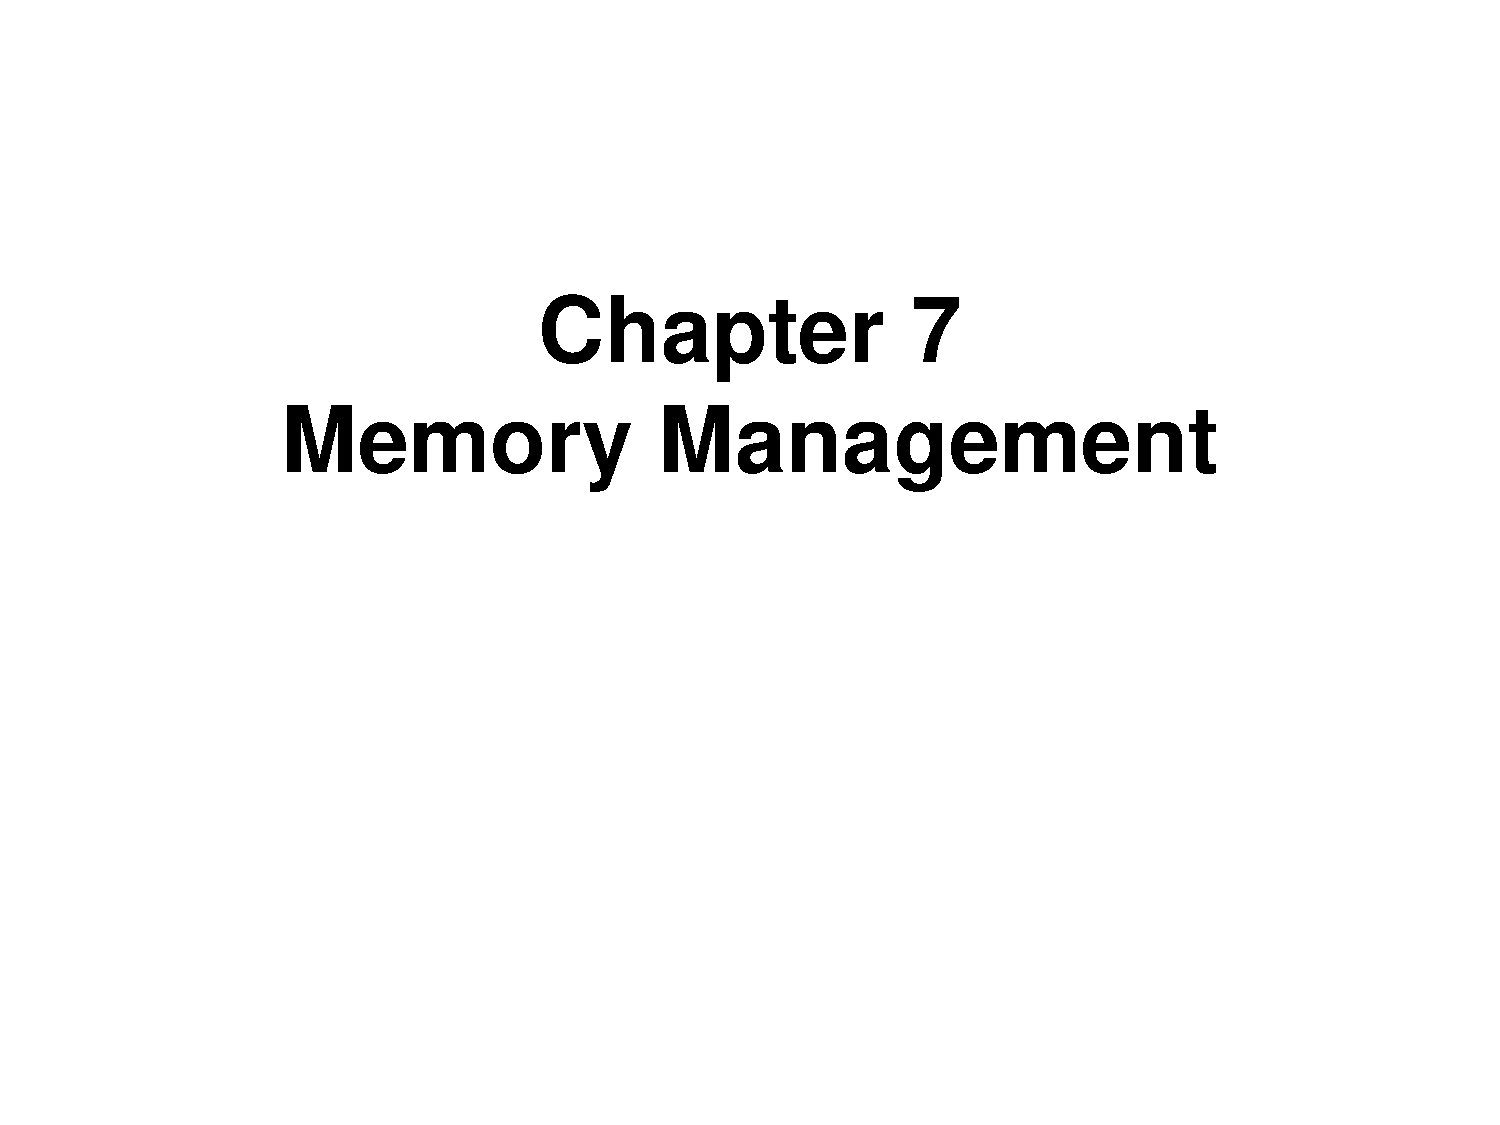
\includepdf[page=21]{07.pdf}
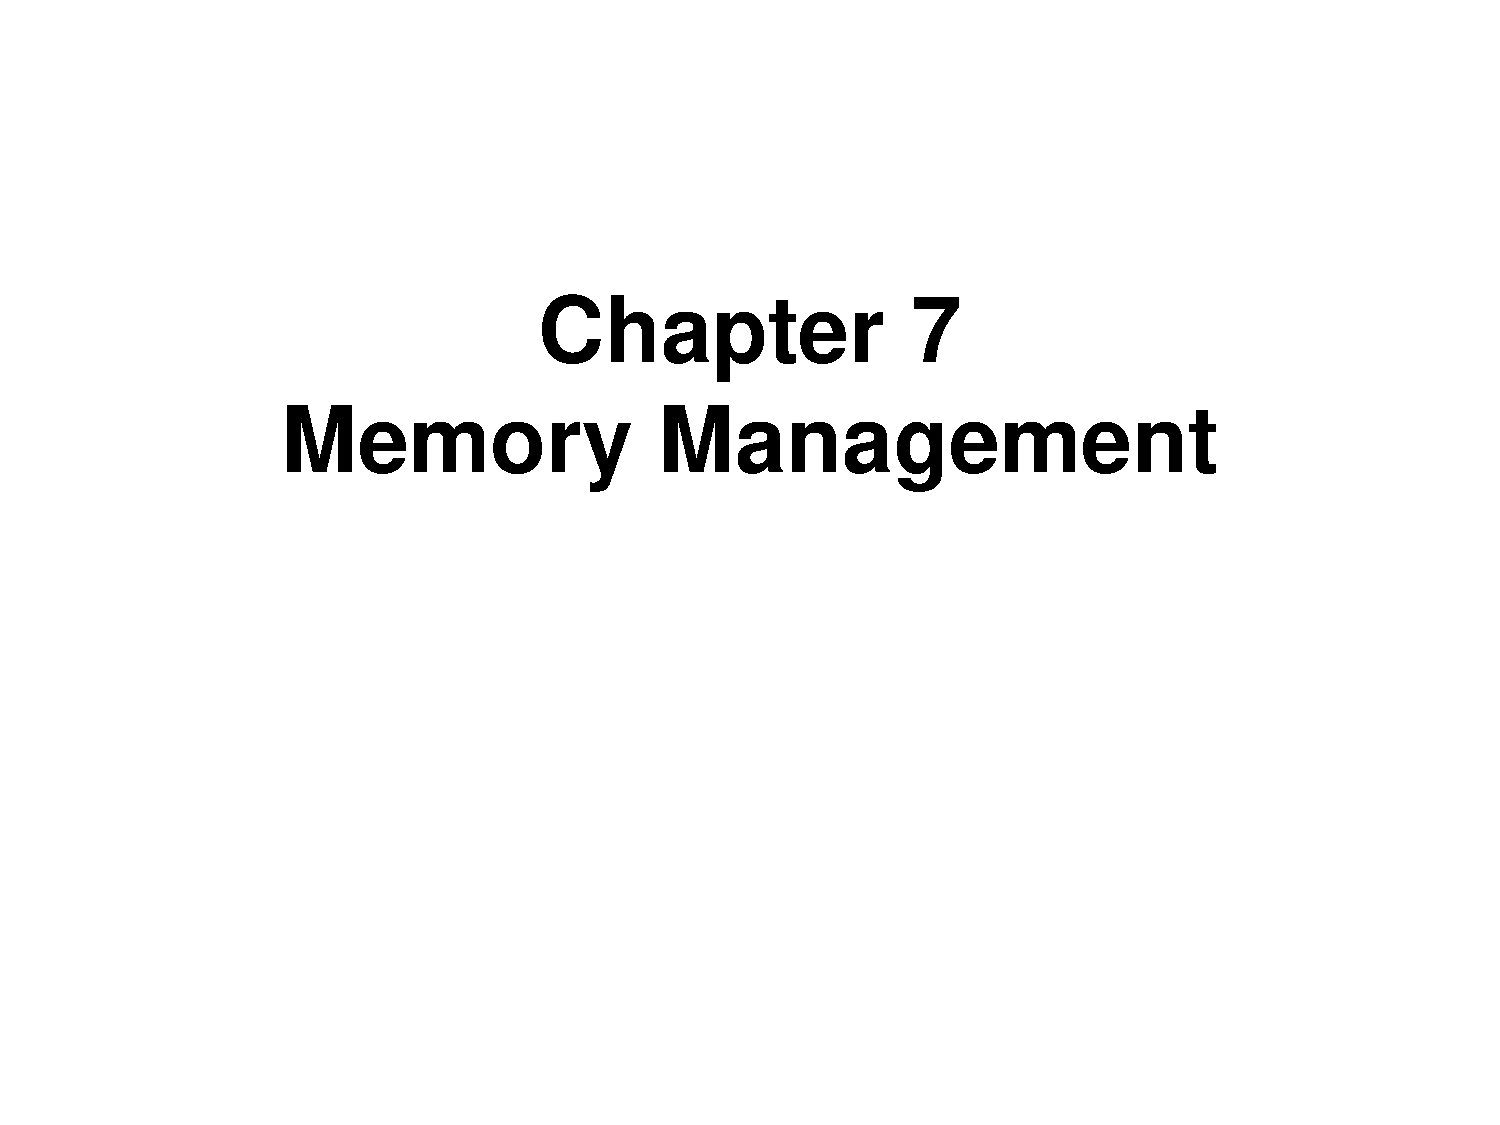
\includepdf[page=22]{07.pdf}
Take all of your memory called $2^u$ always want the size of our process to be $2^{u-1} < s \leq 2^u$. This becomes a recursive algorithm. We keep dividing memory in half until we find a place for the program that fulfills the previous inequality. We keep a tree of allocations, for each level we store them as a list.
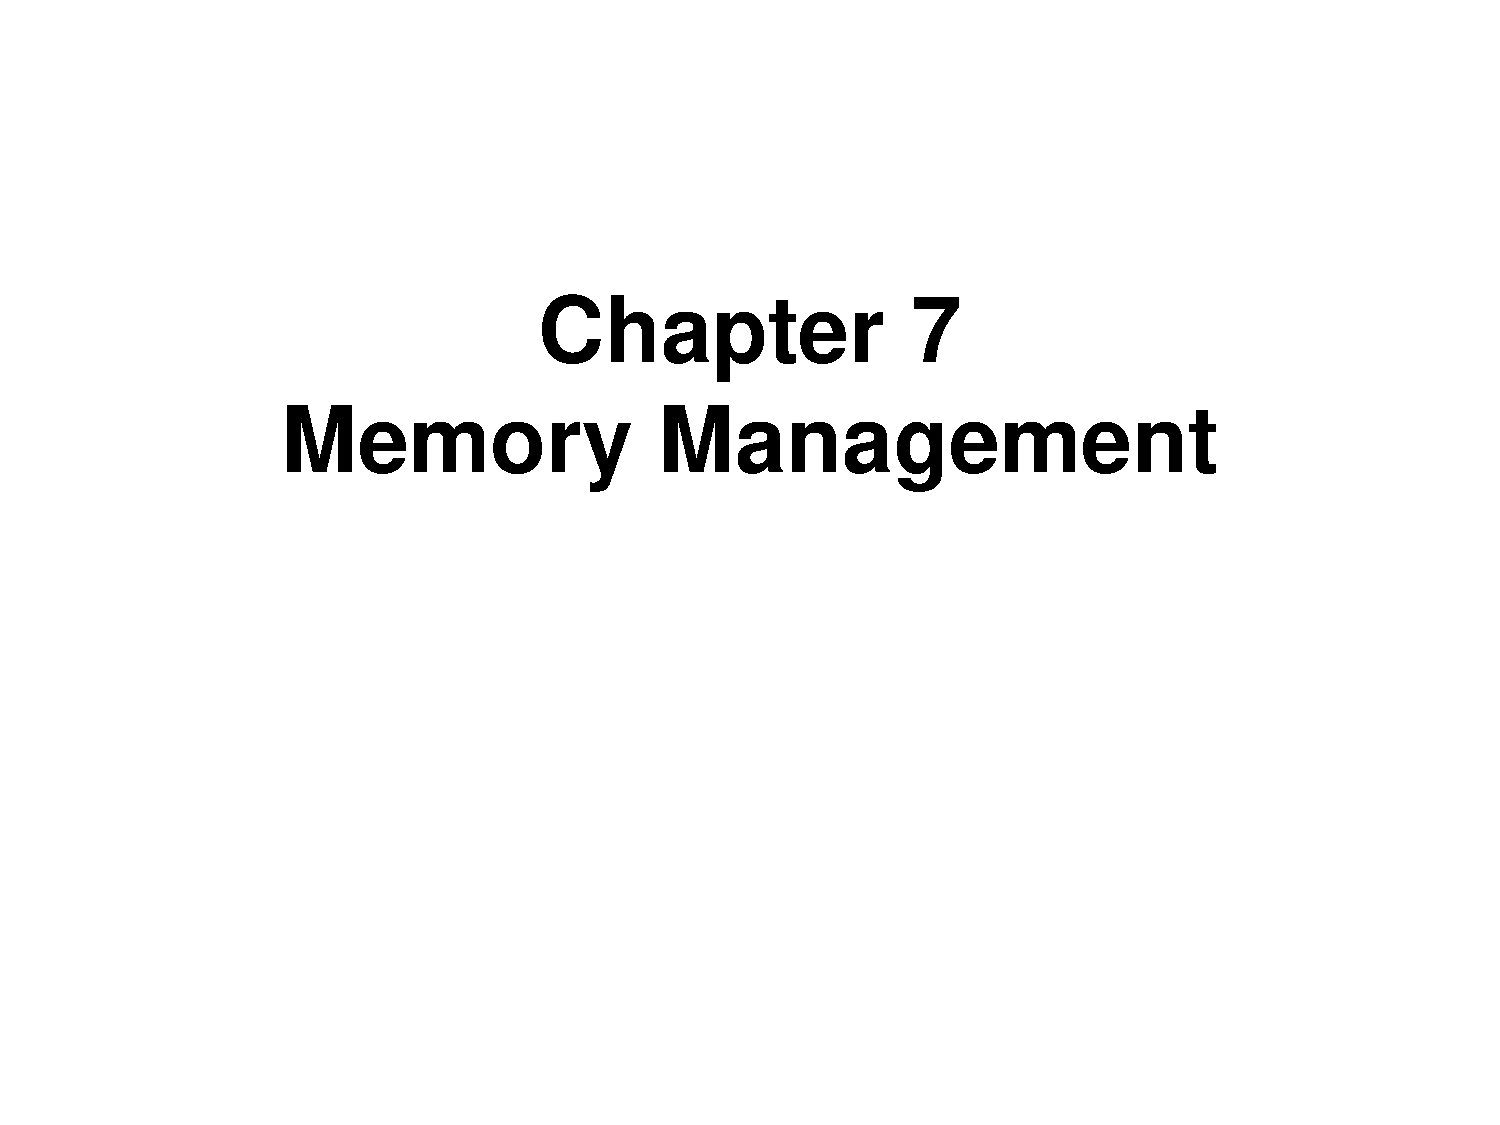
\includepdf[page=23]{07.pdf}
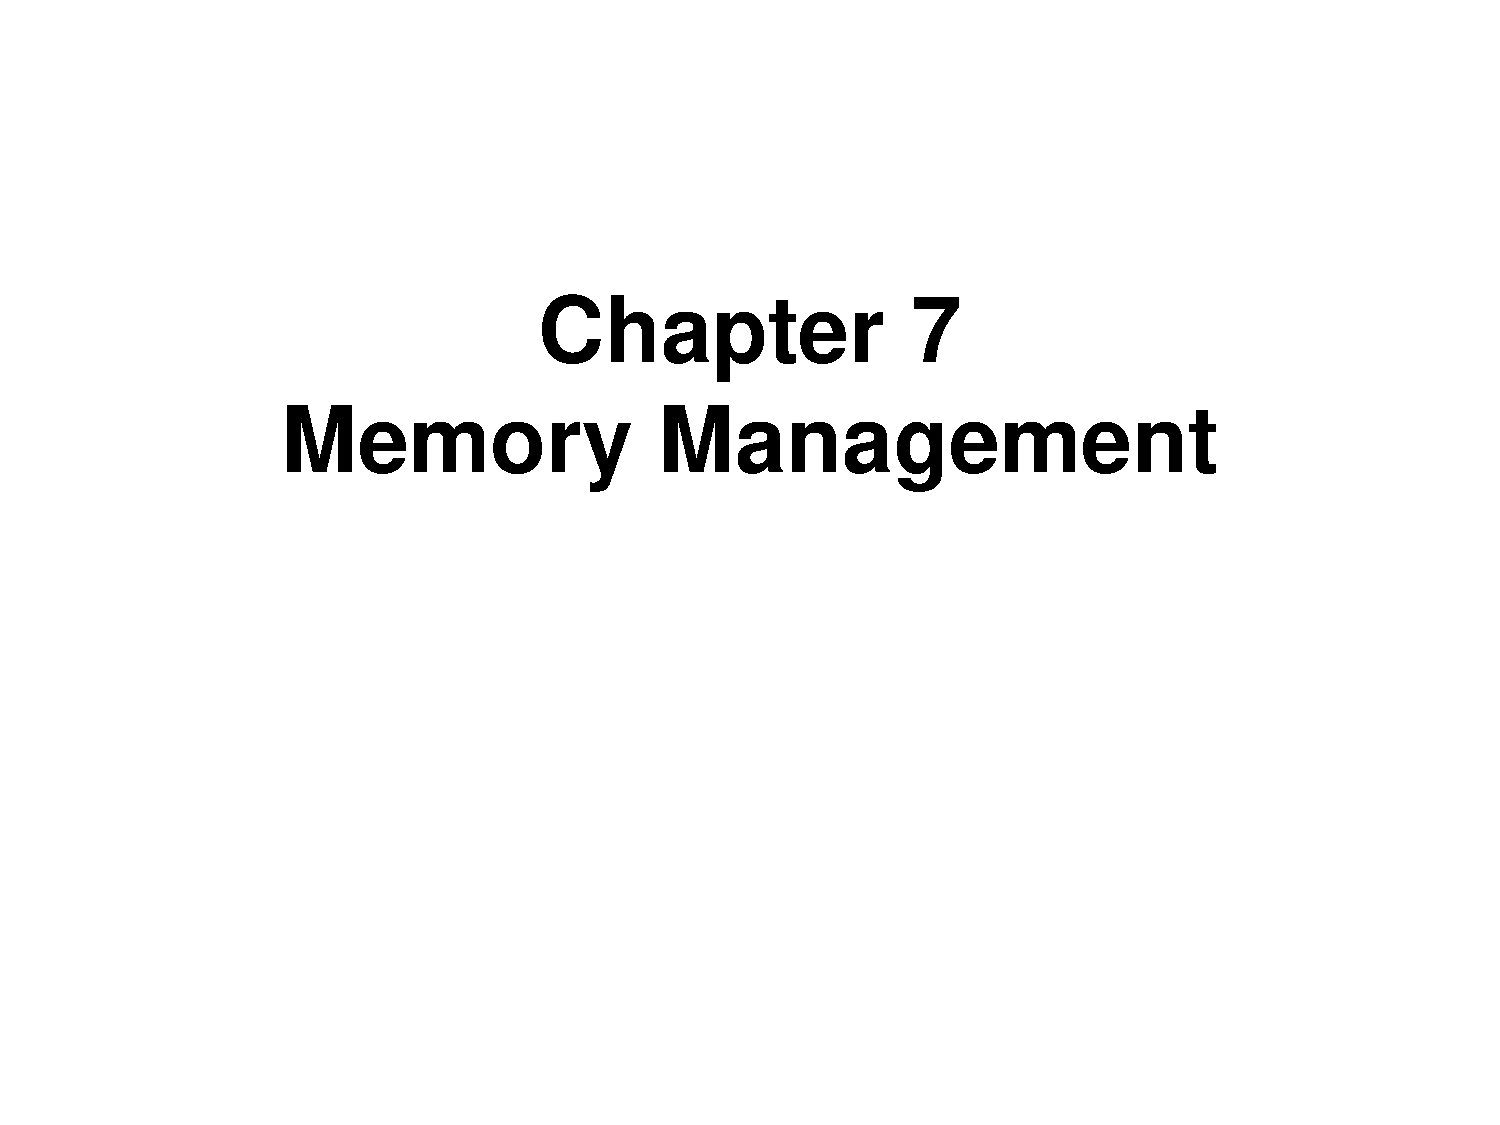
\includepdf[page=24]{07.pdf}
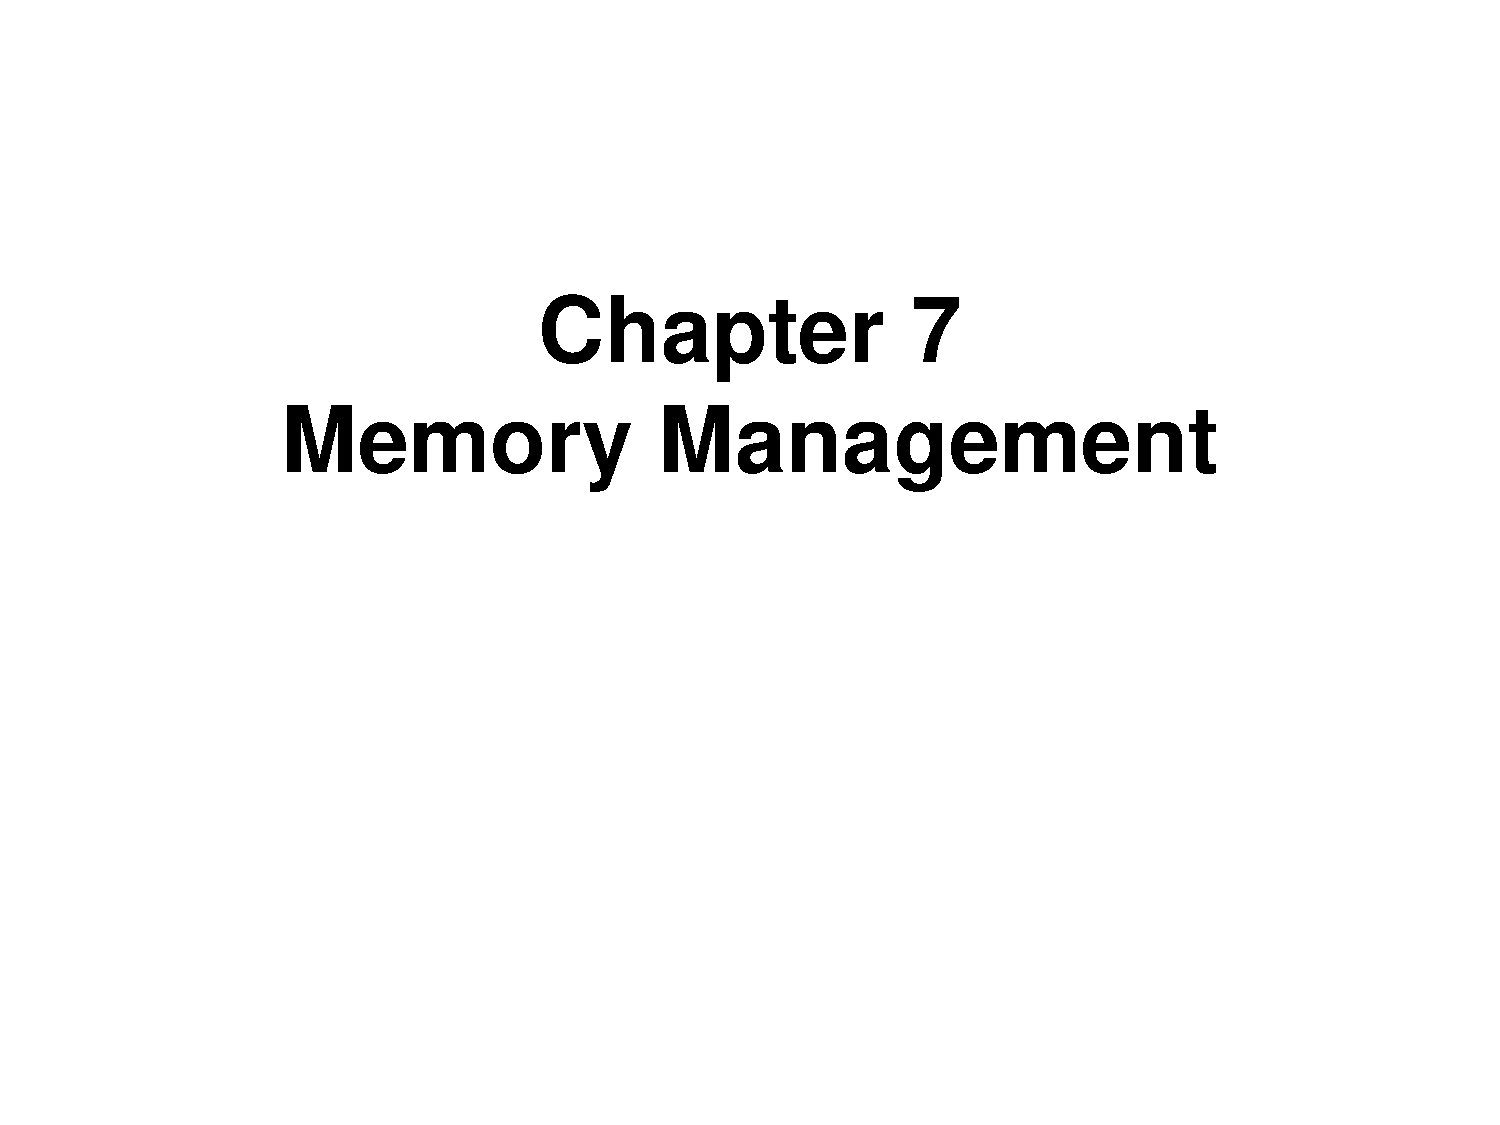
\includepdf[page=25]{07.pdf}
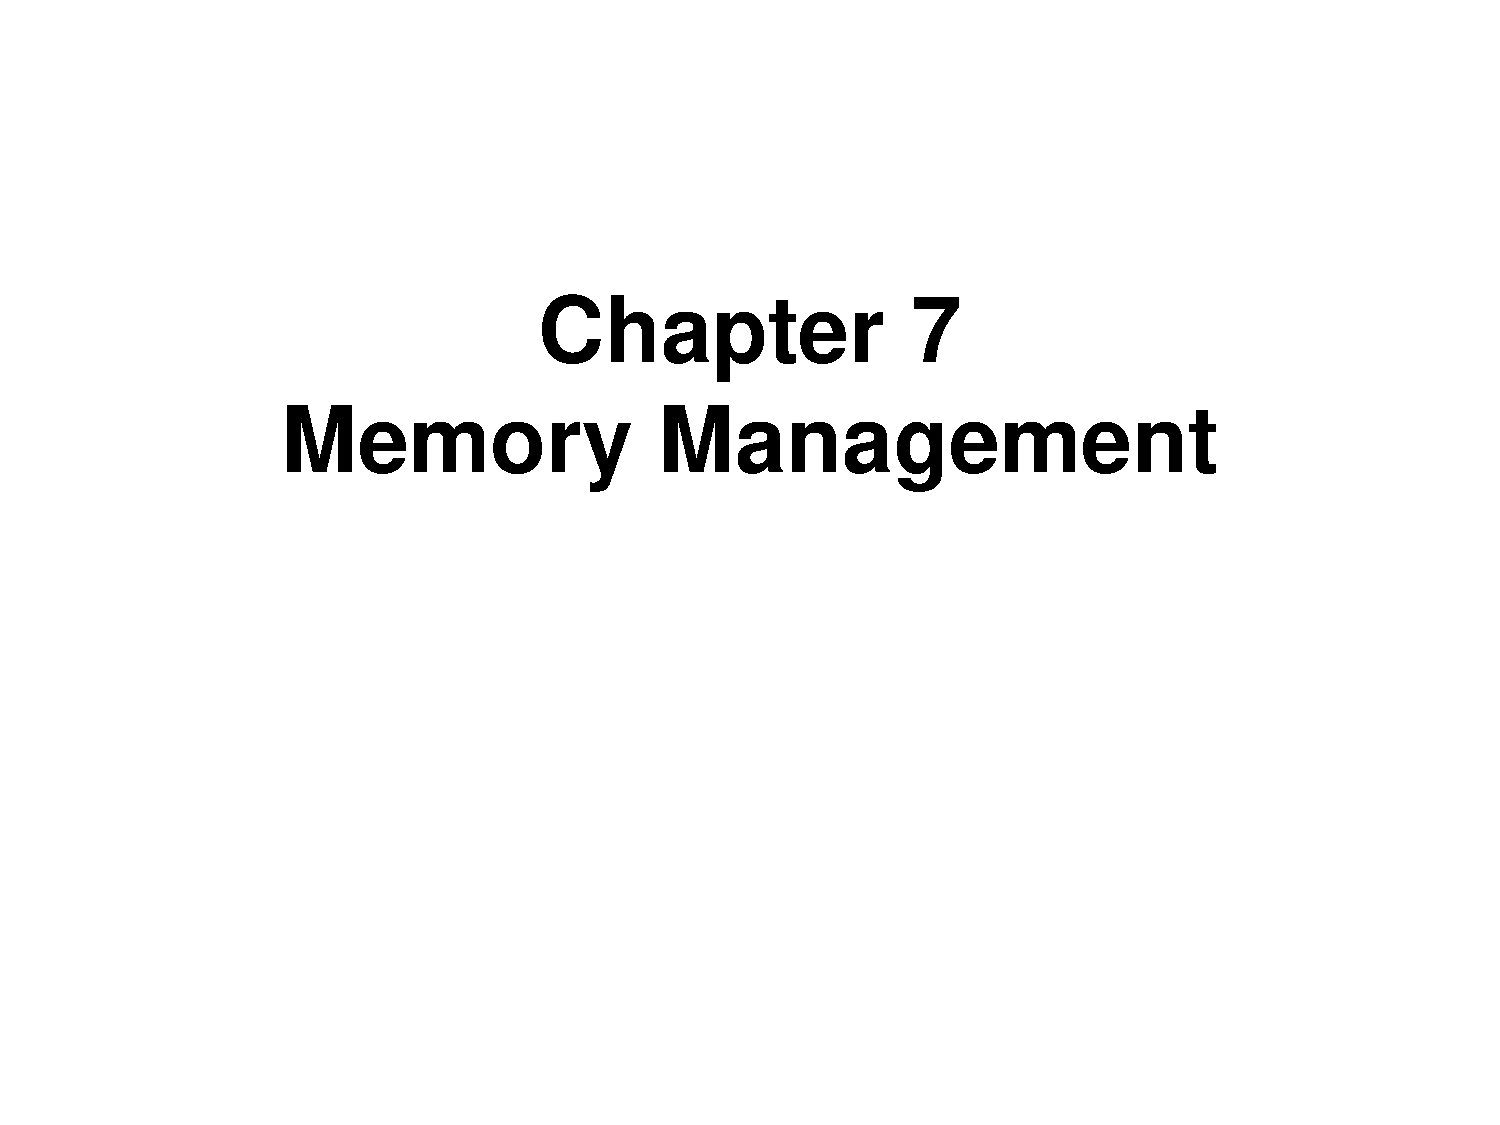
\includepdf[page=26]{07.pdf}
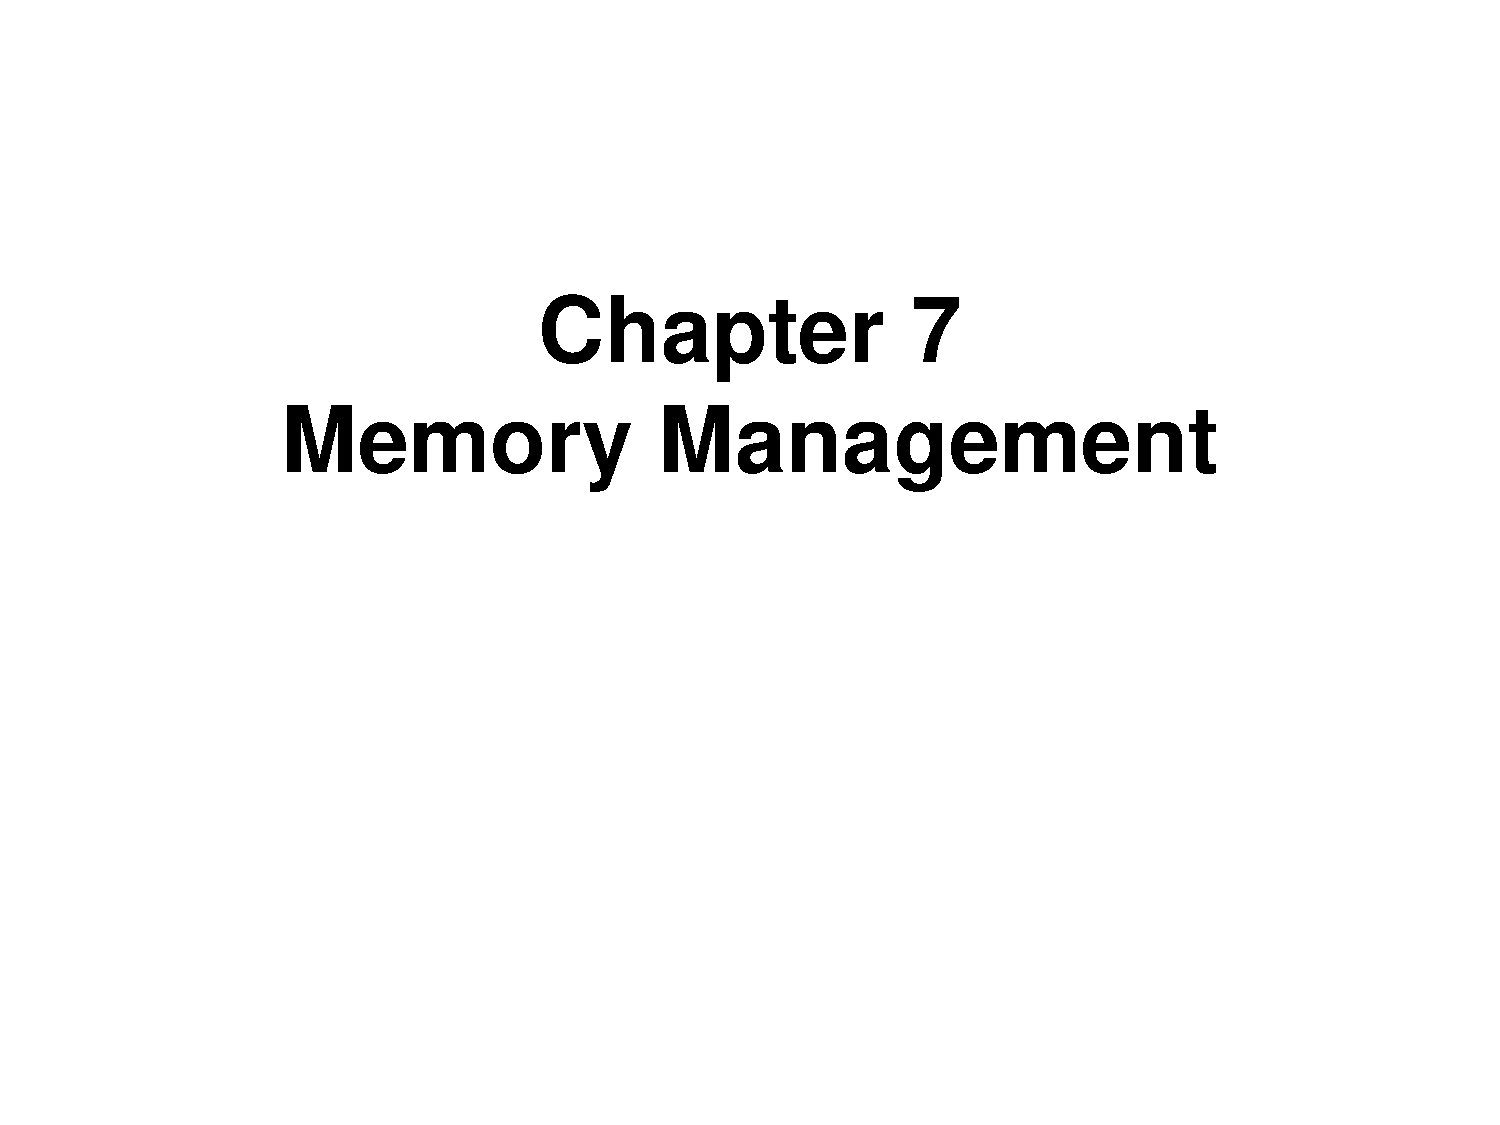
\includepdf[page=27]{07.pdf}
When we map out the addresses we have some references in the program image which is local address and some absolute address in local space where the memory resides whichch we need to implement. We need to add a base register where it was loaded and a bounds register which marks its limits. The adder and comparter are turning the local addresses into valid addresses at run time.
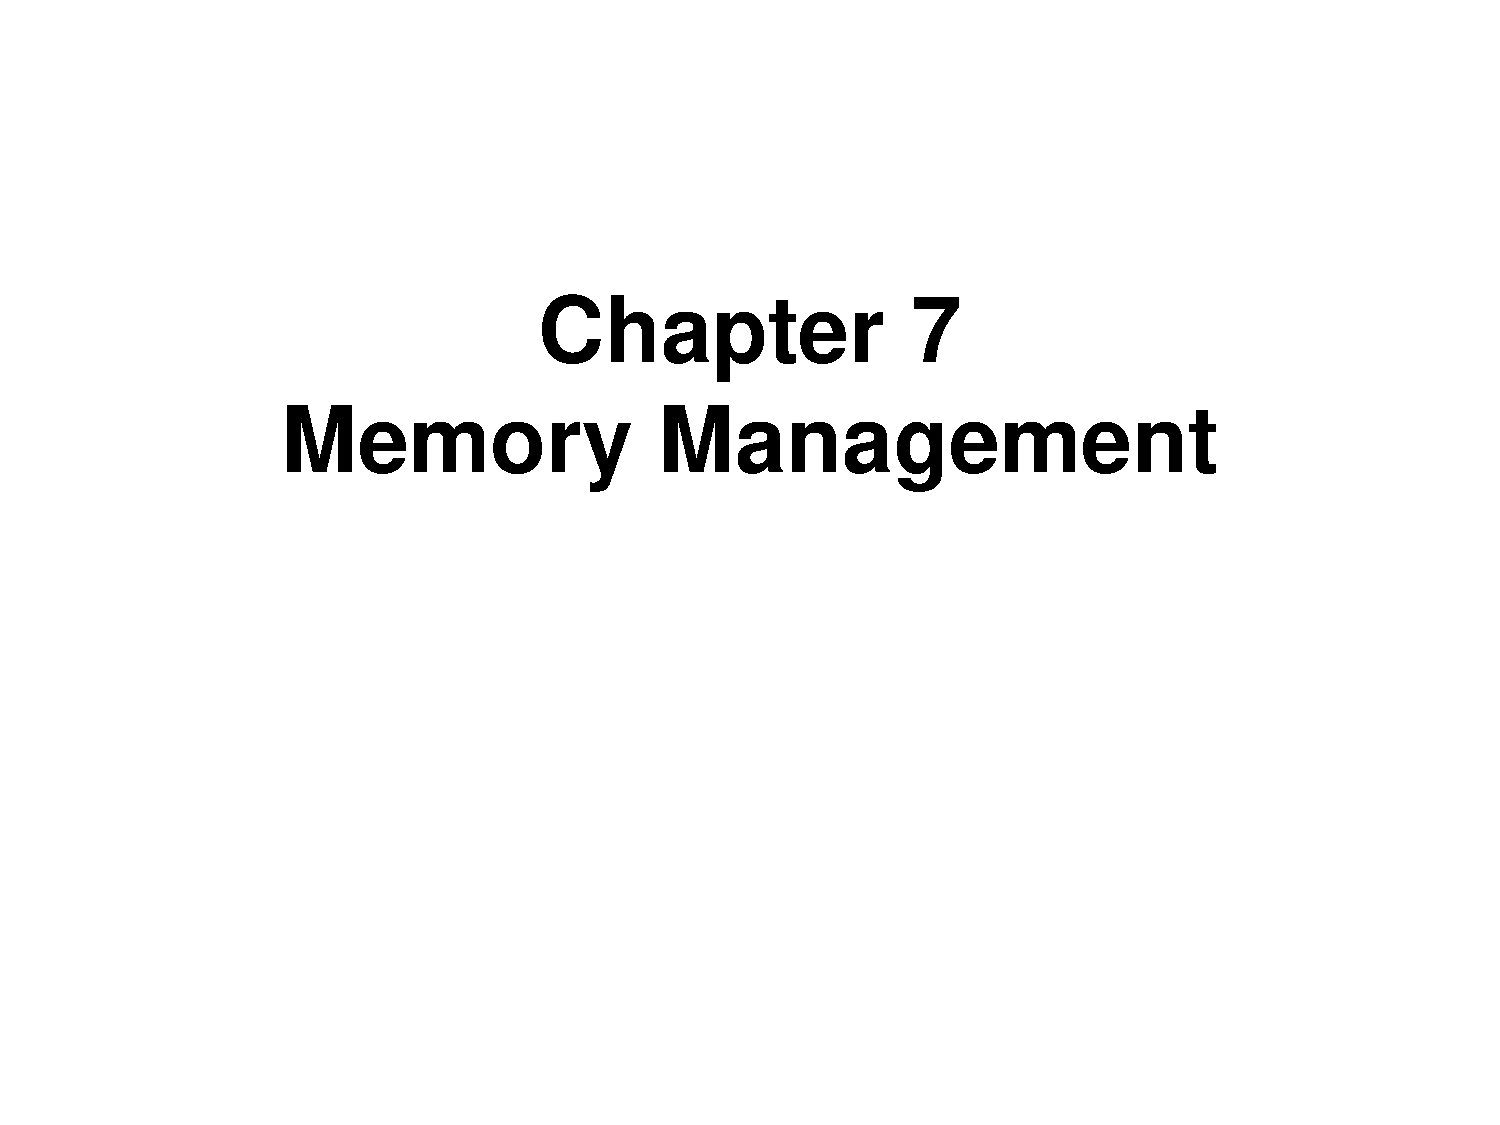
\includepdf[page=28]{07.pdf}
The registers used for house keeping (where the process is and the relative addresses used) are stored in the process control block
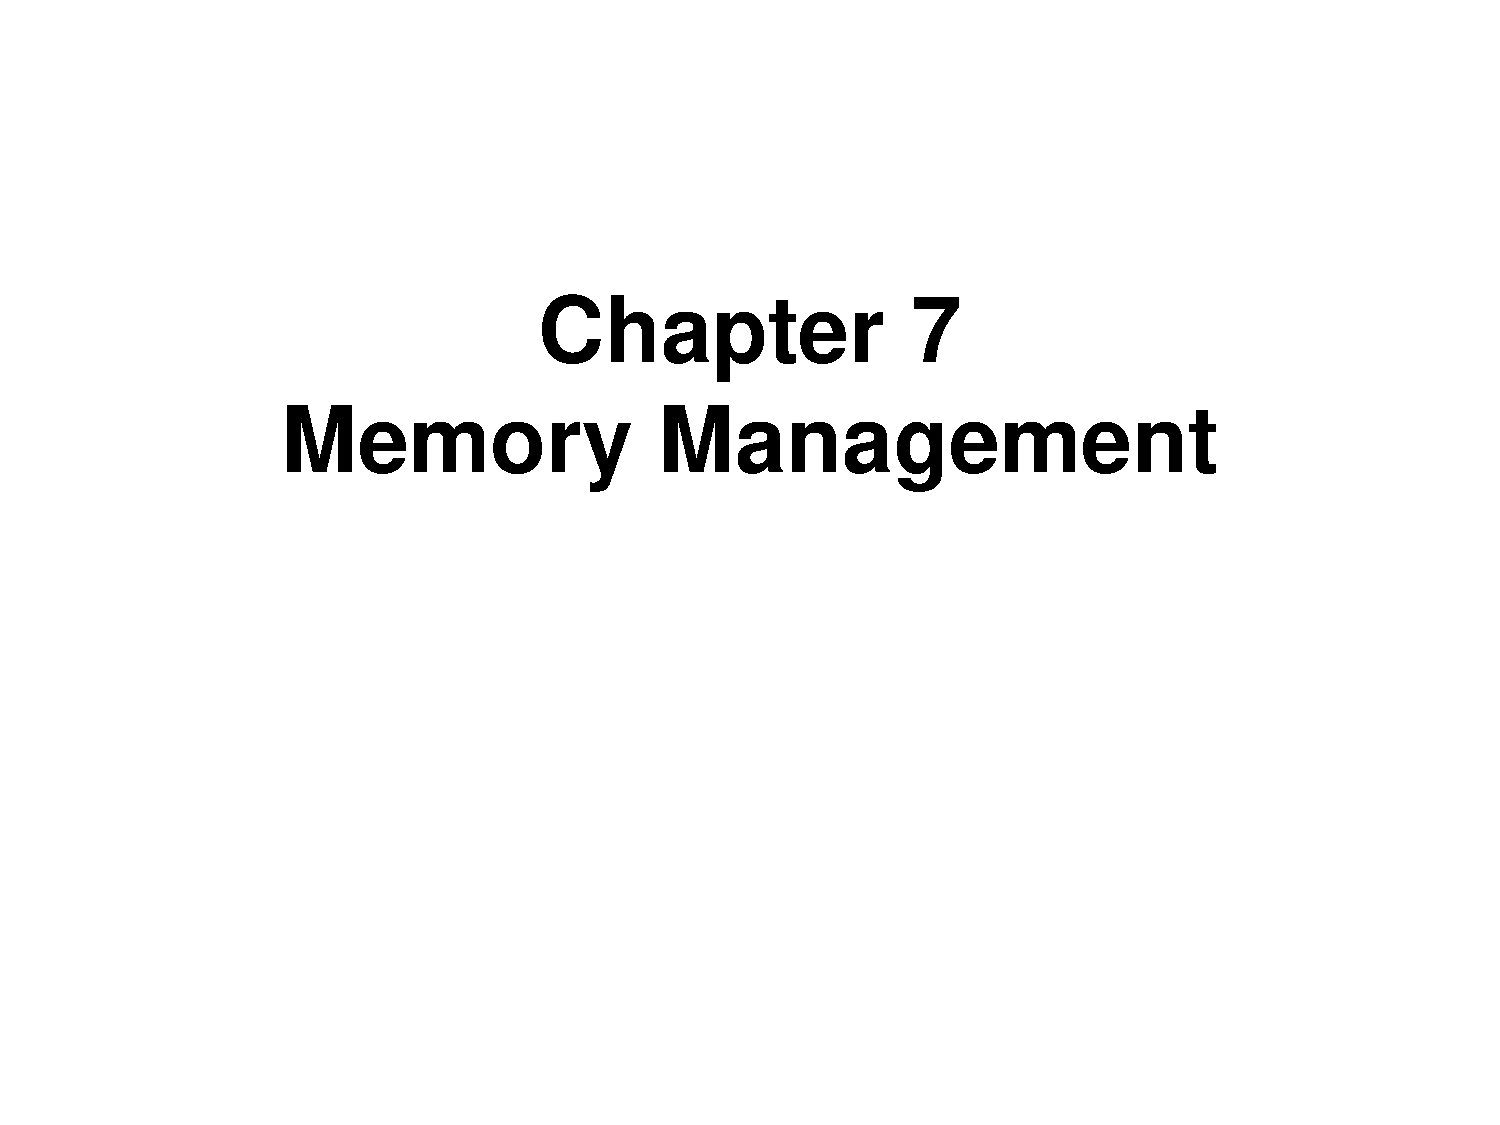
\includepdf[page=29]{07.pdf}
This is a good concept to remember to know how it works on a high level. The hardware implementation is much more sophistocated. Relocation in the context of fragmetation gets much more complicated.
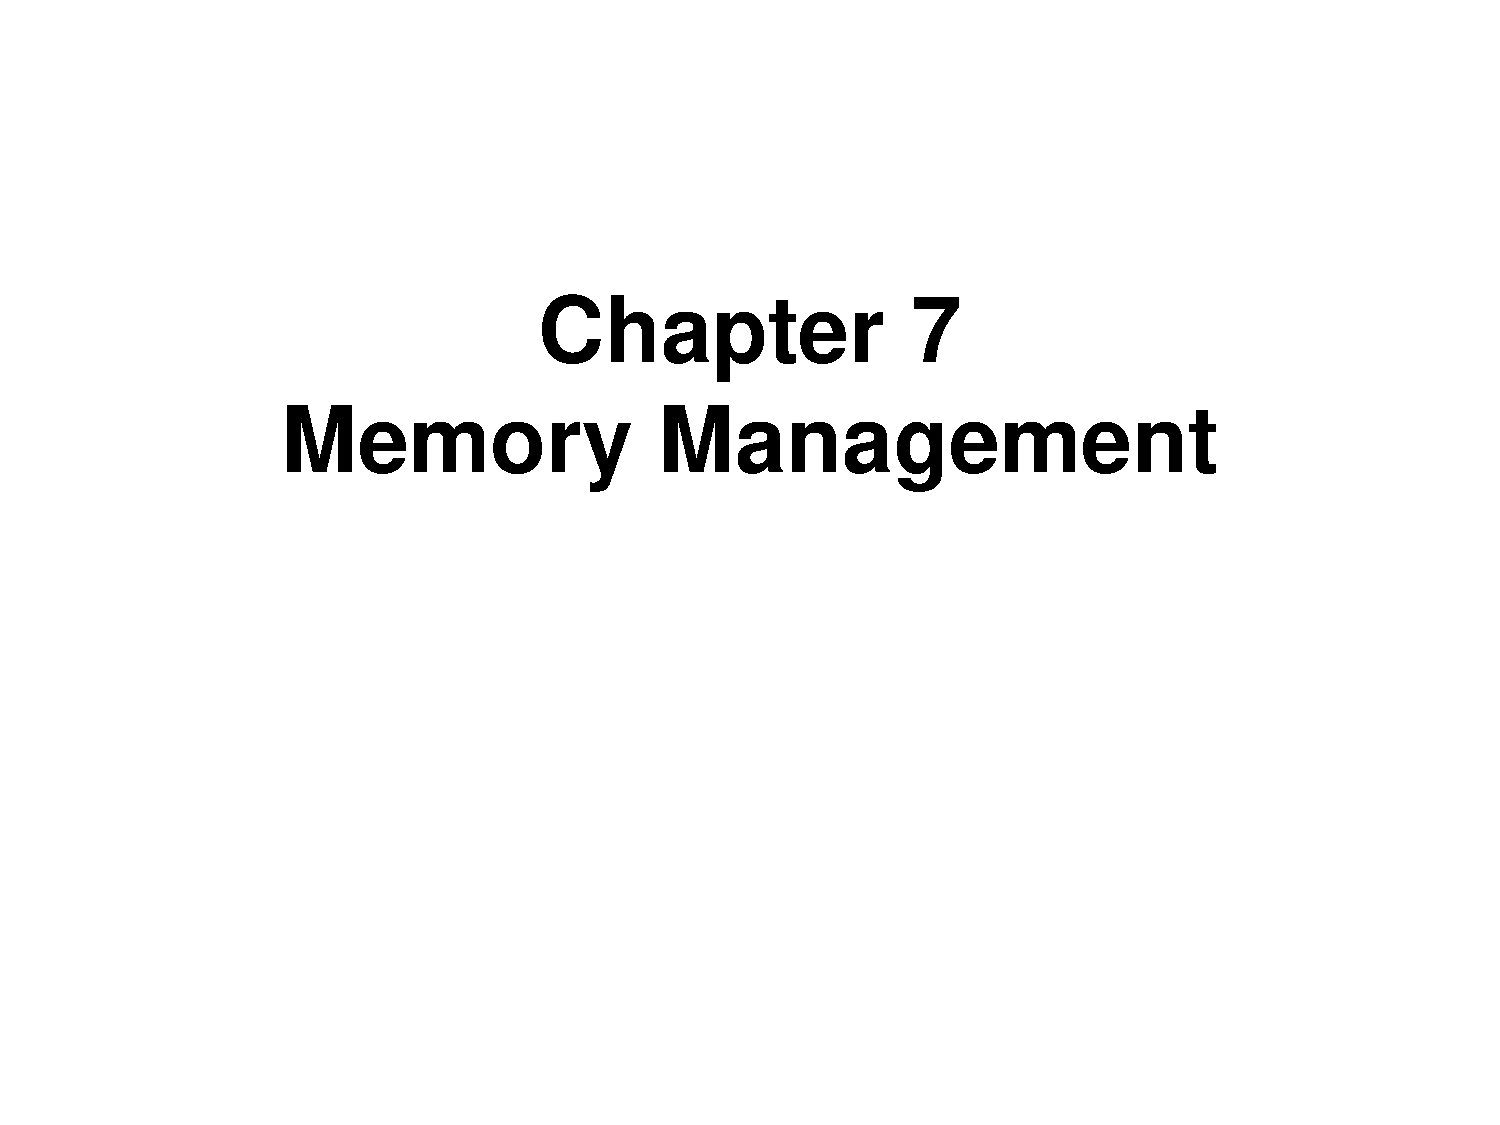
\includepdf[page=30]{07.pdf}
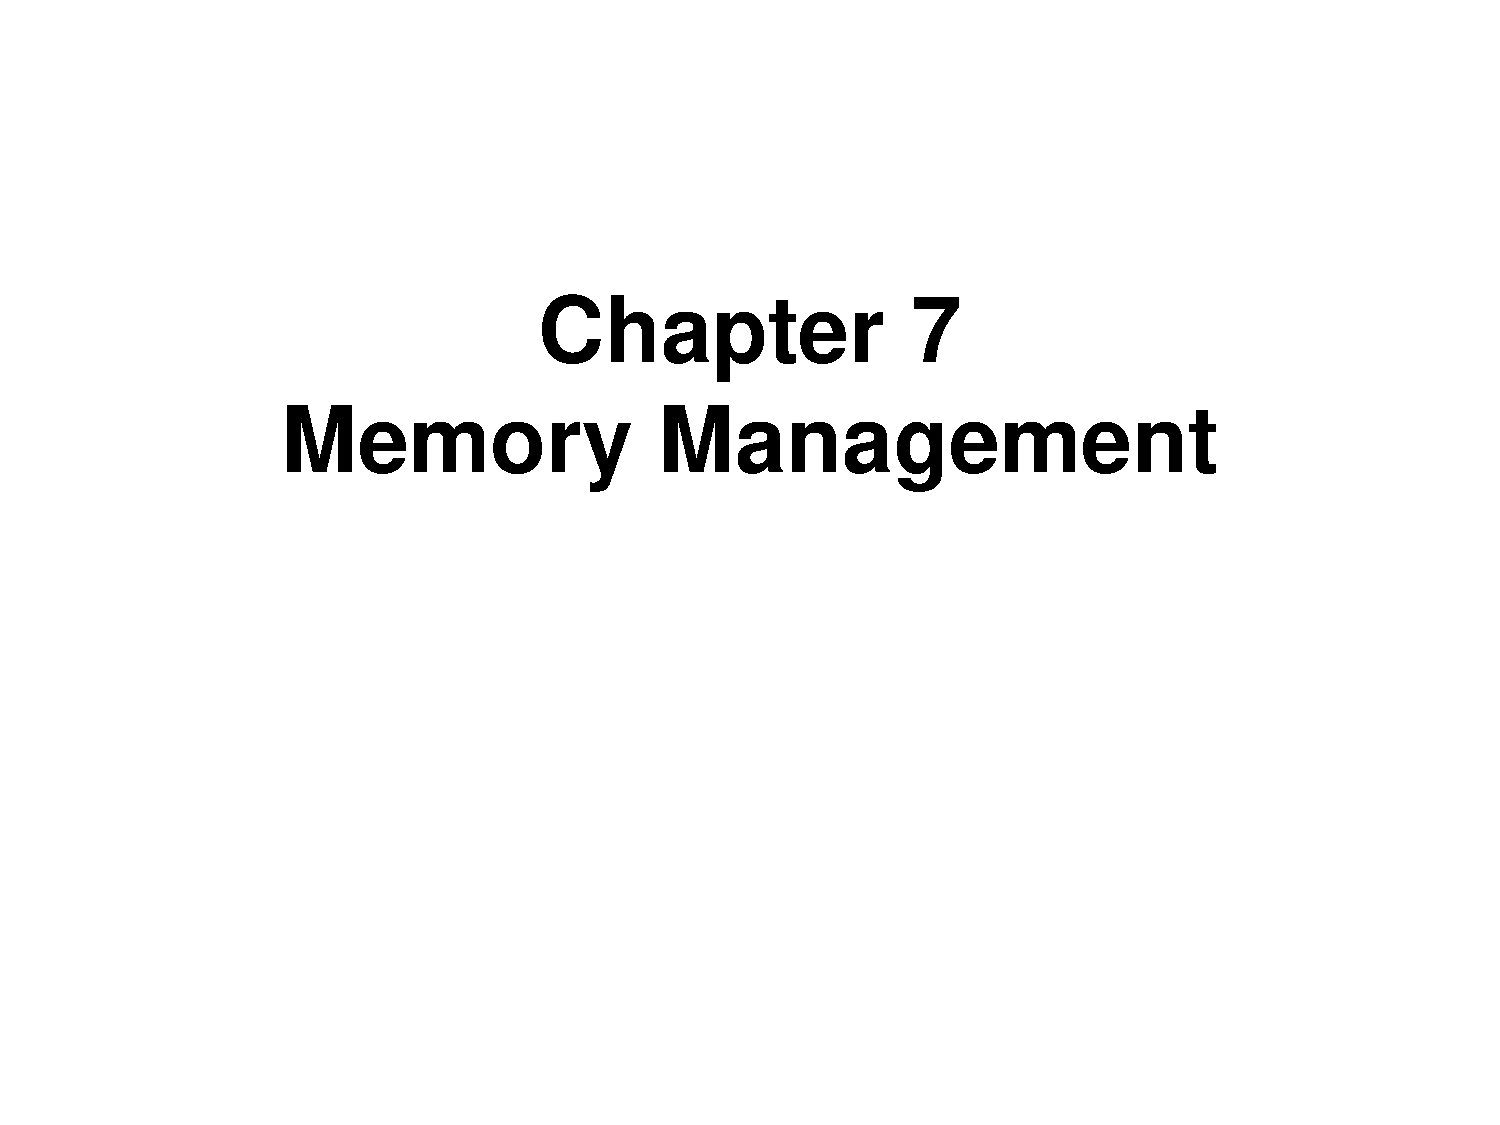
\includepdf[page=31]{07.pdf}
Break your process image into equal sized chunks called pages. Load each page into a frame (chunk of ram) and updates the pointer to it.
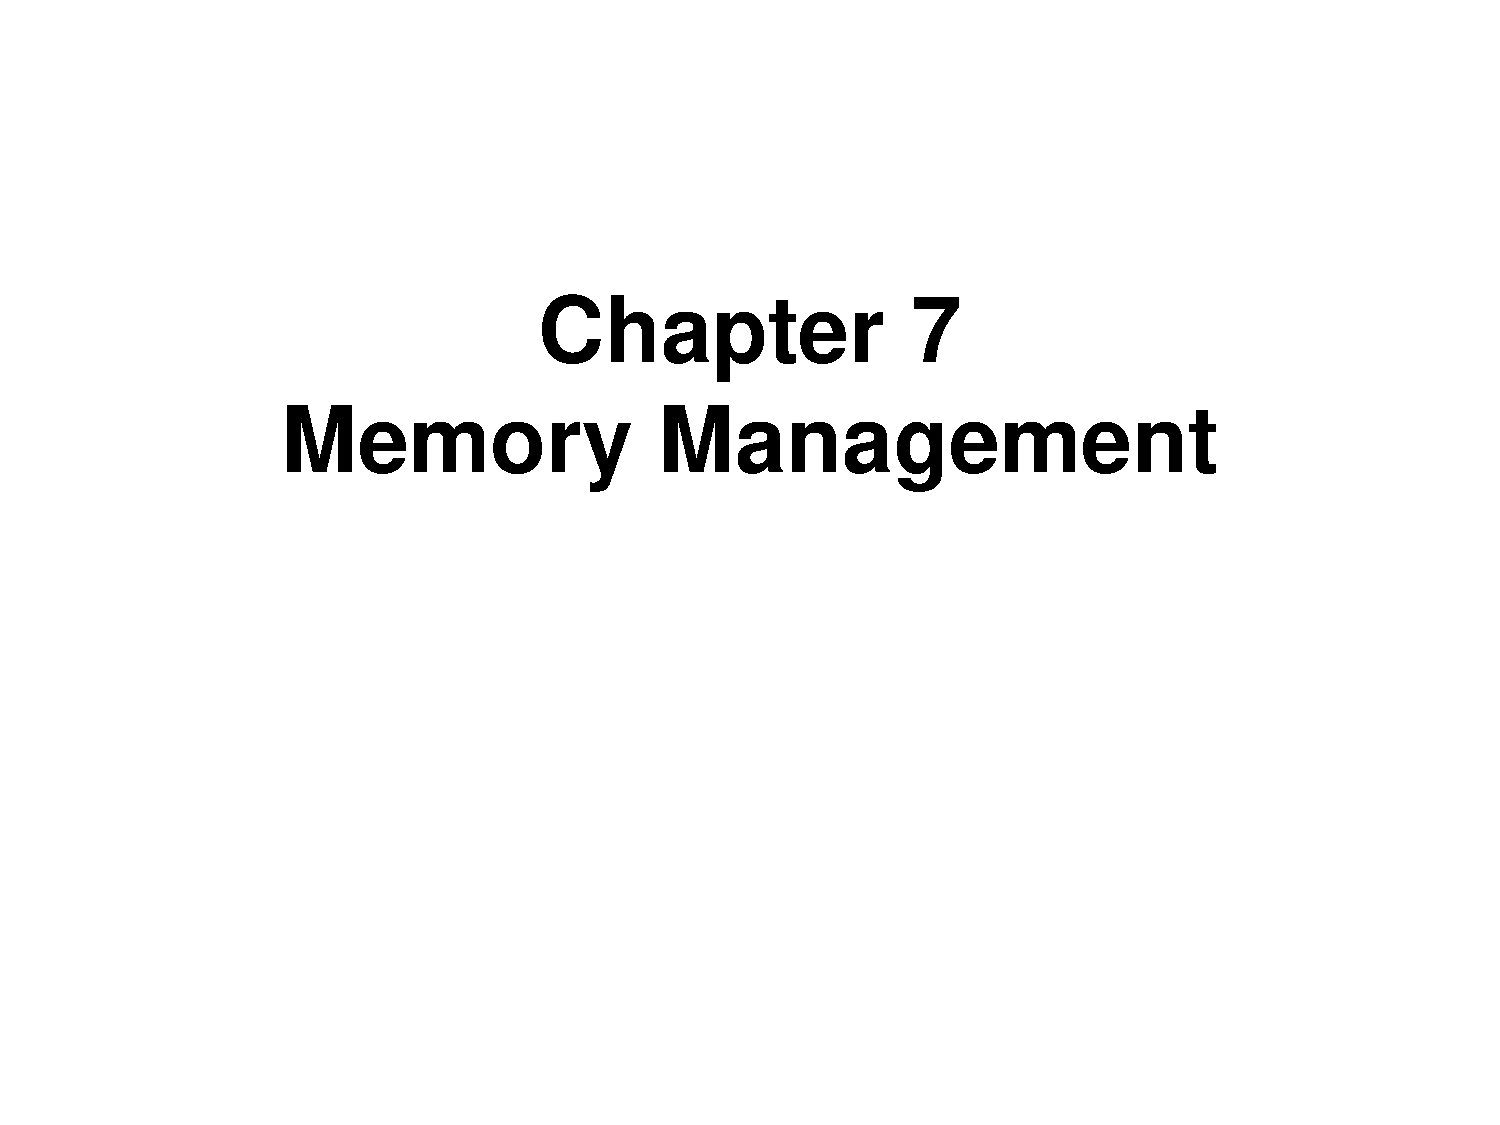
\includepdf[page=32]{07.pdf}
We keep track of the mapping of pages to main memory. We translate the offset of a value in the program image to a address in the associated frame.

We reserve a chunk of real memory that stores your memory table (mapping). Every time we switch processes we get the page address from the PCB and load that into memory for use. We need to make sure that the memory table doesn't get erased or changed. We can nest paging tables.
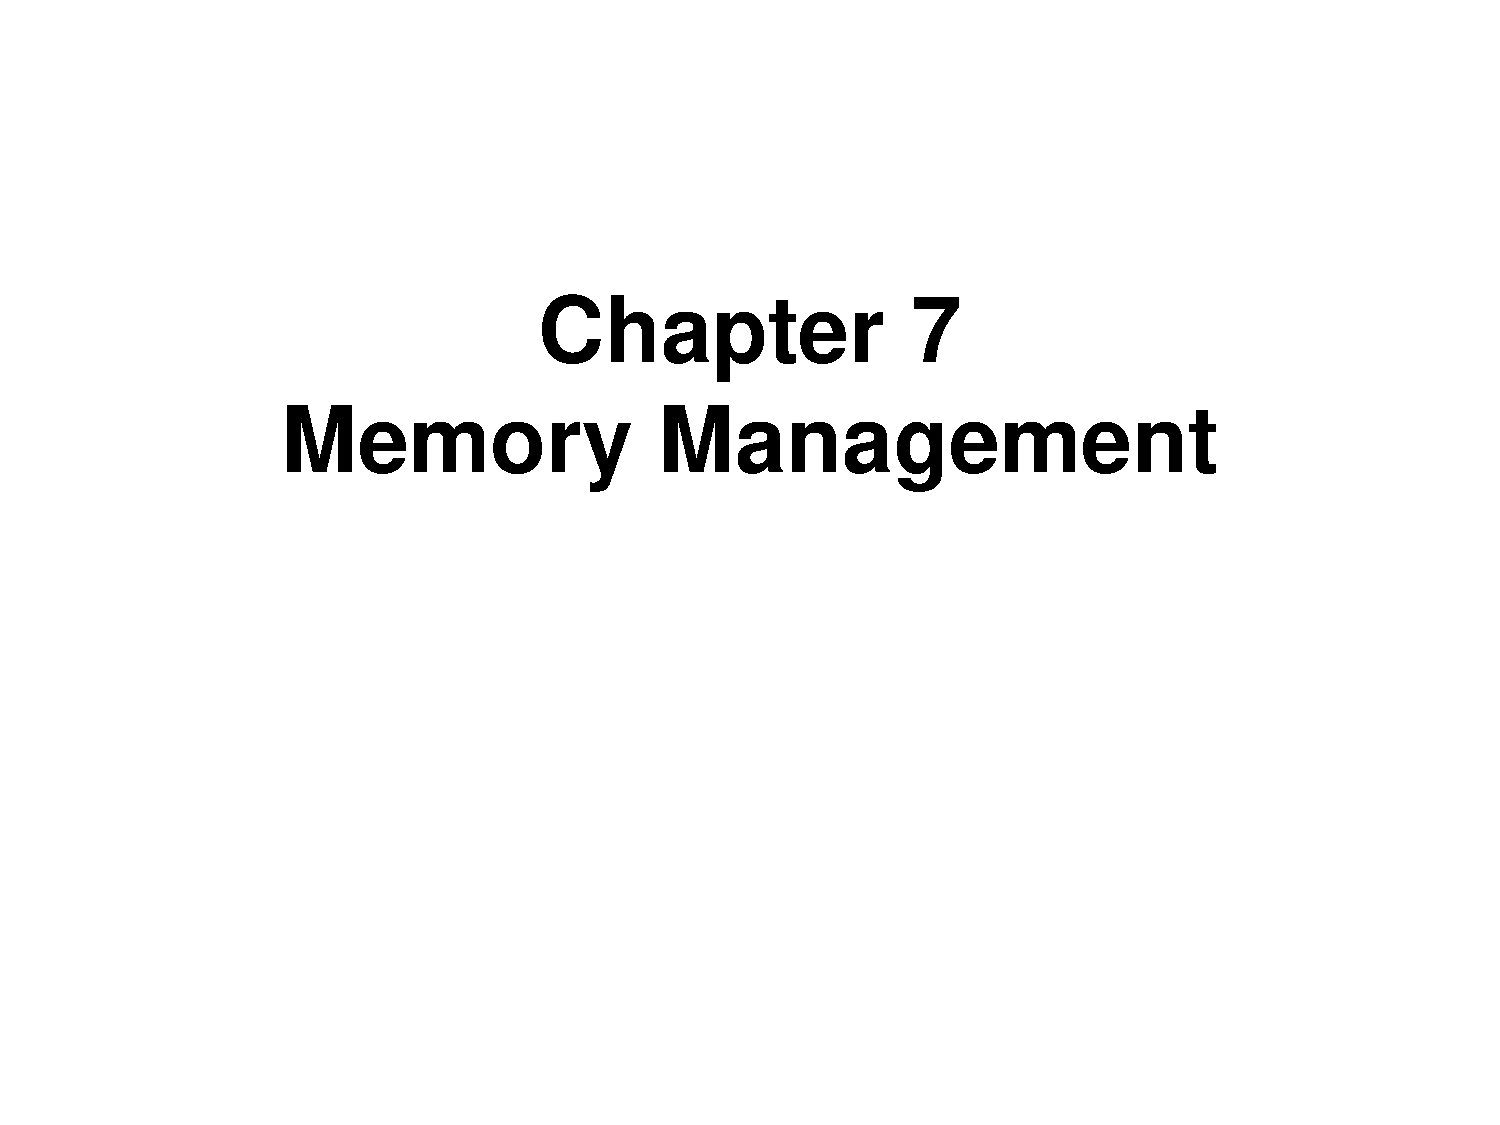
\includepdf[page=33]{07.pdf}
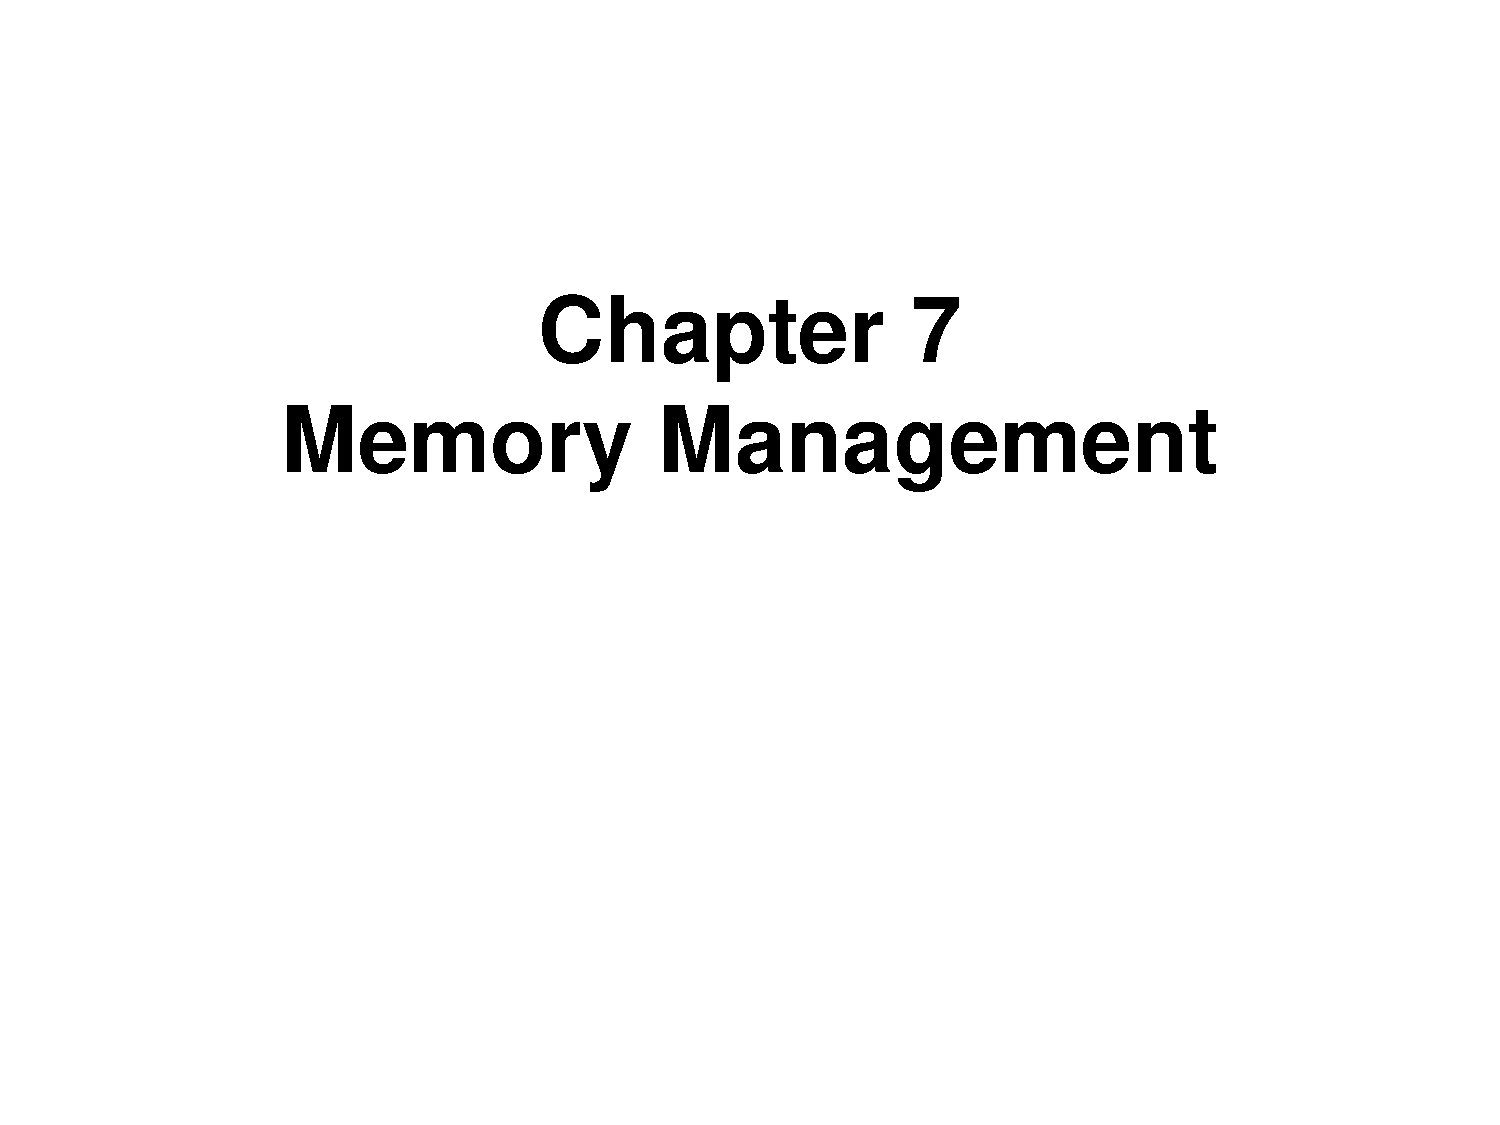
\includepdf[page=34]{07.pdf}
Here we can allocate 5 frames since the memory doesnt have to be continuous.
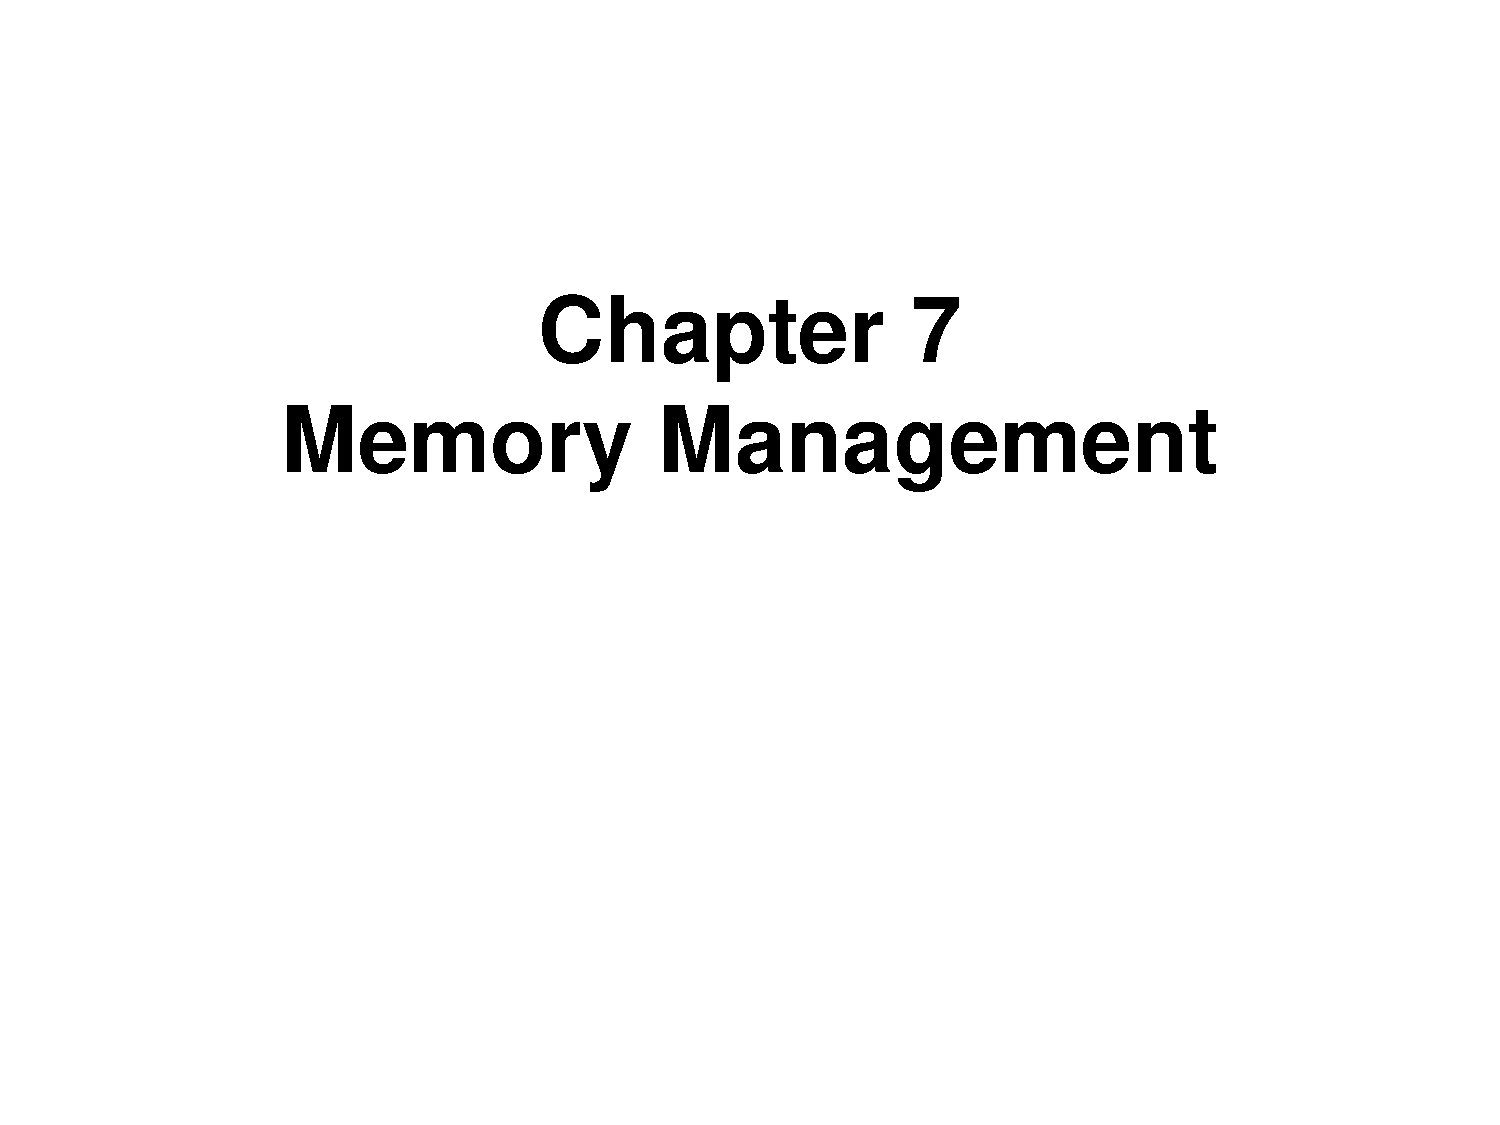
\includepdf[page=35]{07.pdf}
Here we see the page mapping where process D is not continuous.
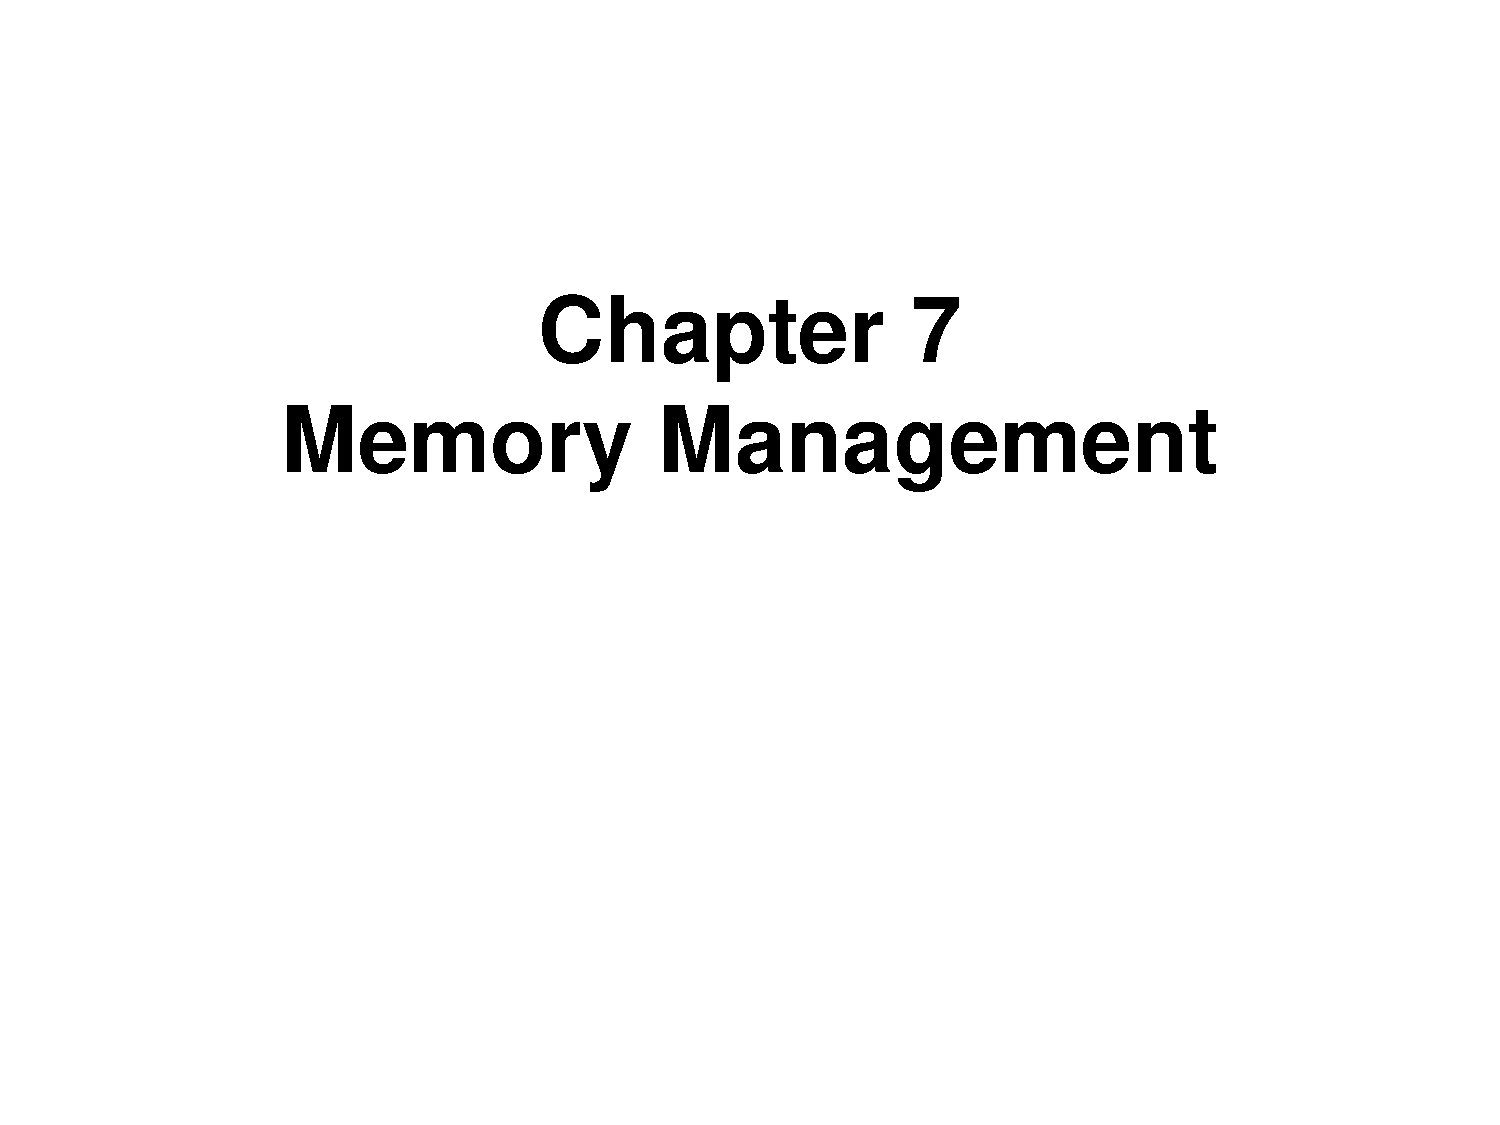
\includepdf[page=36]{07.pdf}
Instead of dividing memory into equal size blocks have the block size be variable. We refer to a segment number and an offset in that segment.
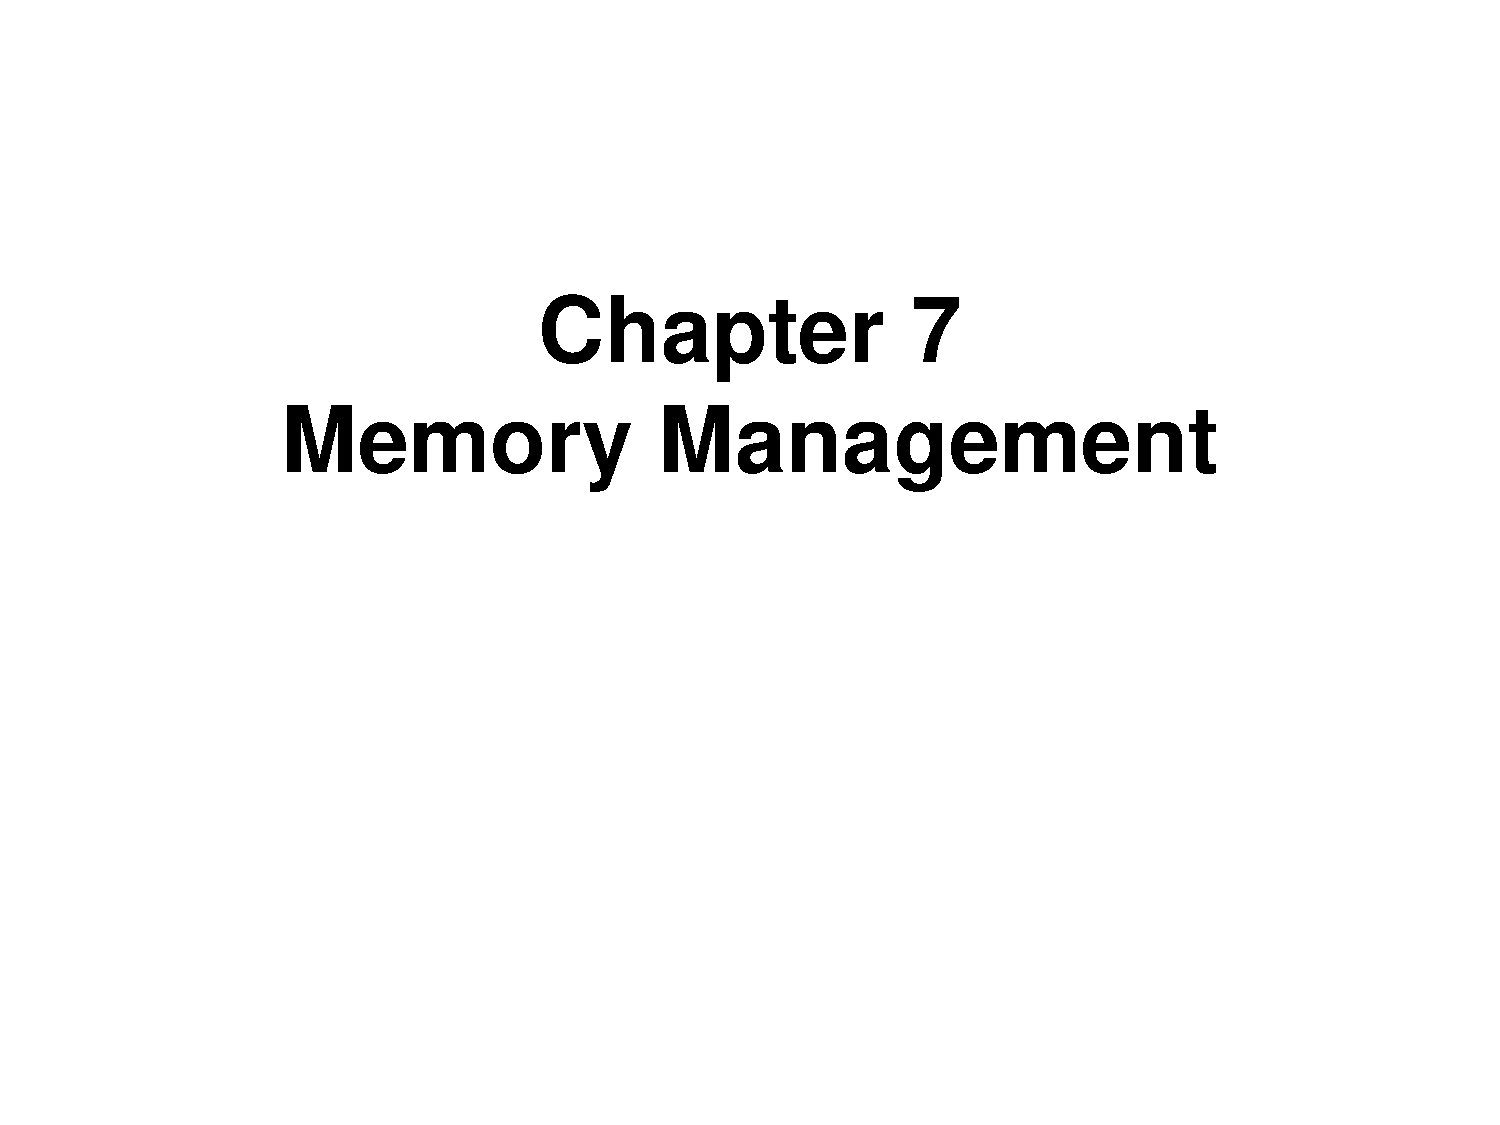
\includepdf[page=37]{07.pdf}
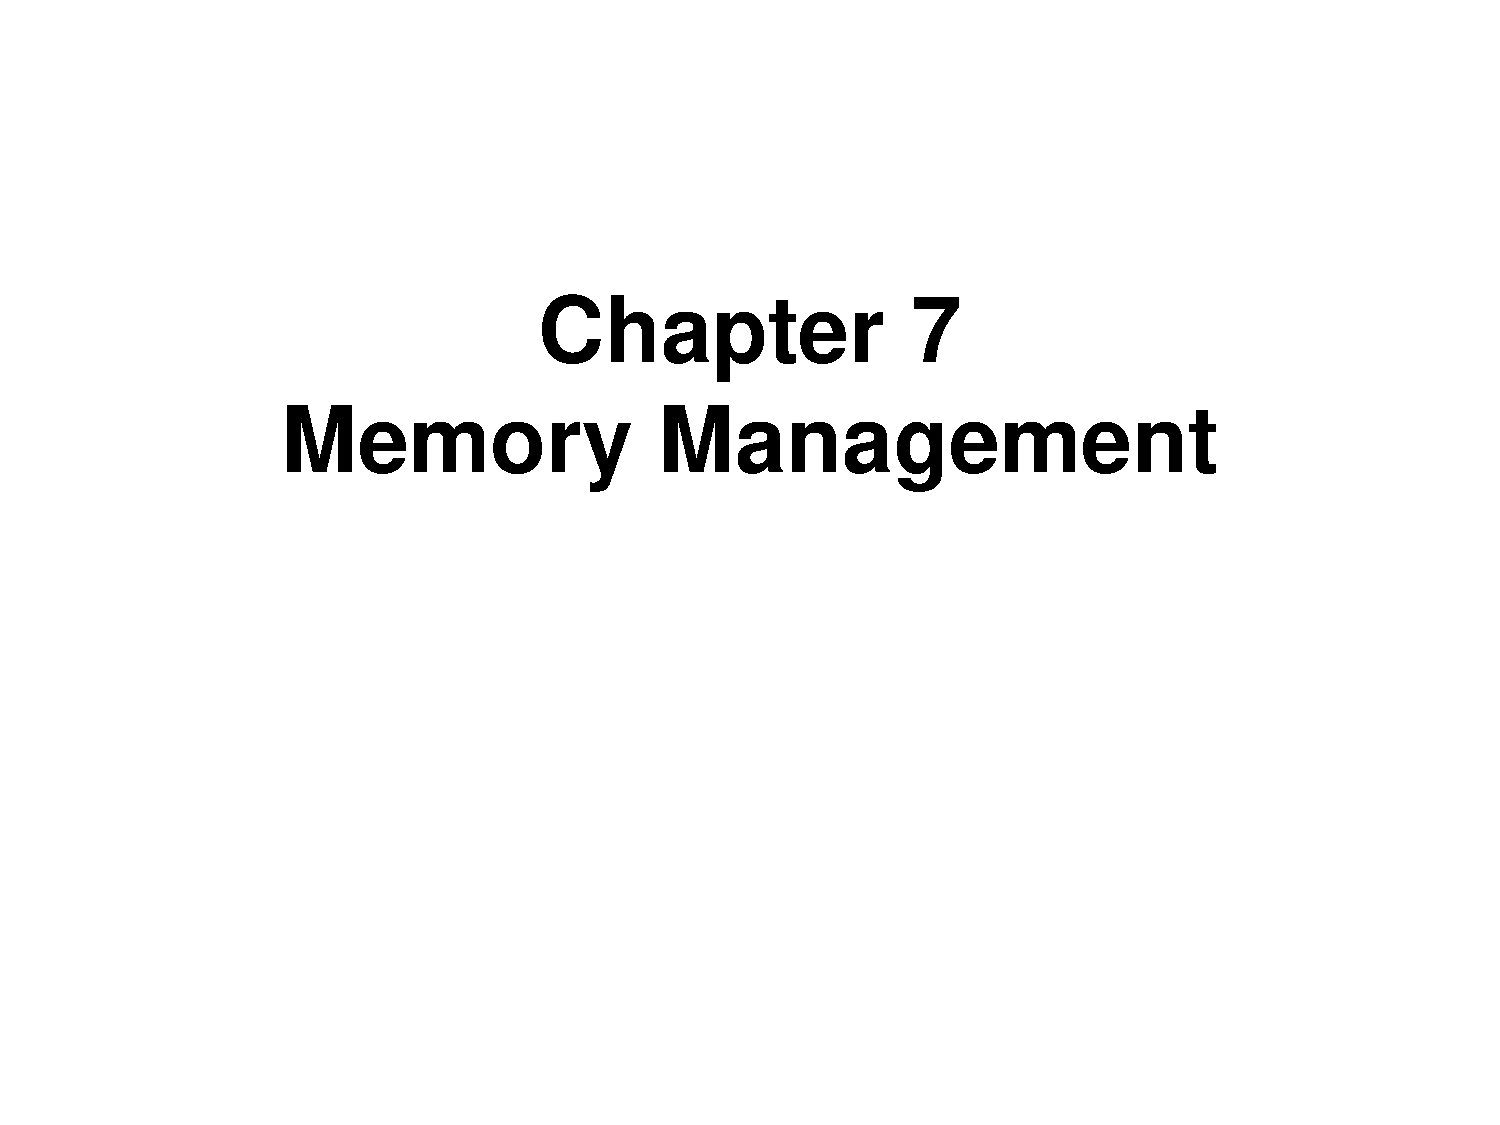
\includepdf[page=38]{07.pdf}
Calculate the most significate bits of the offset and switch them out with the frame. We then copy over the ten bit offset to make a new physical address in the correct segment with the correct offset. The size of the offset determines the size of your page and the page number tells you how many pages you have.
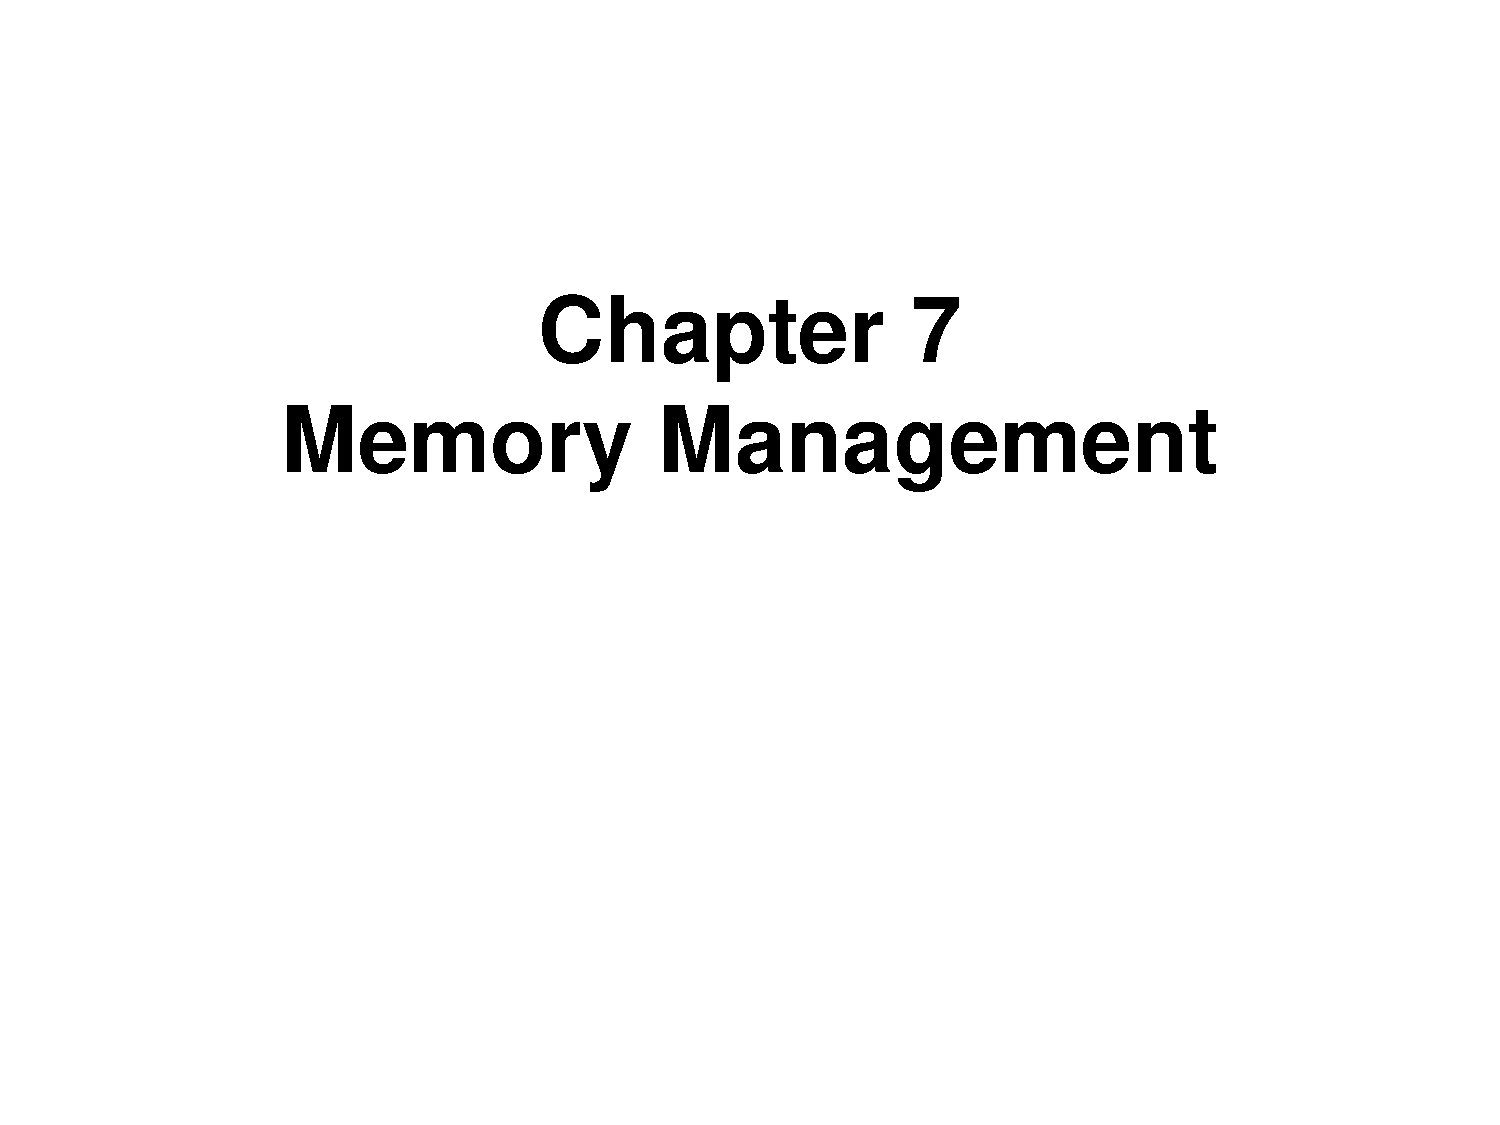
\includepdf[page=39]{07.pdf}
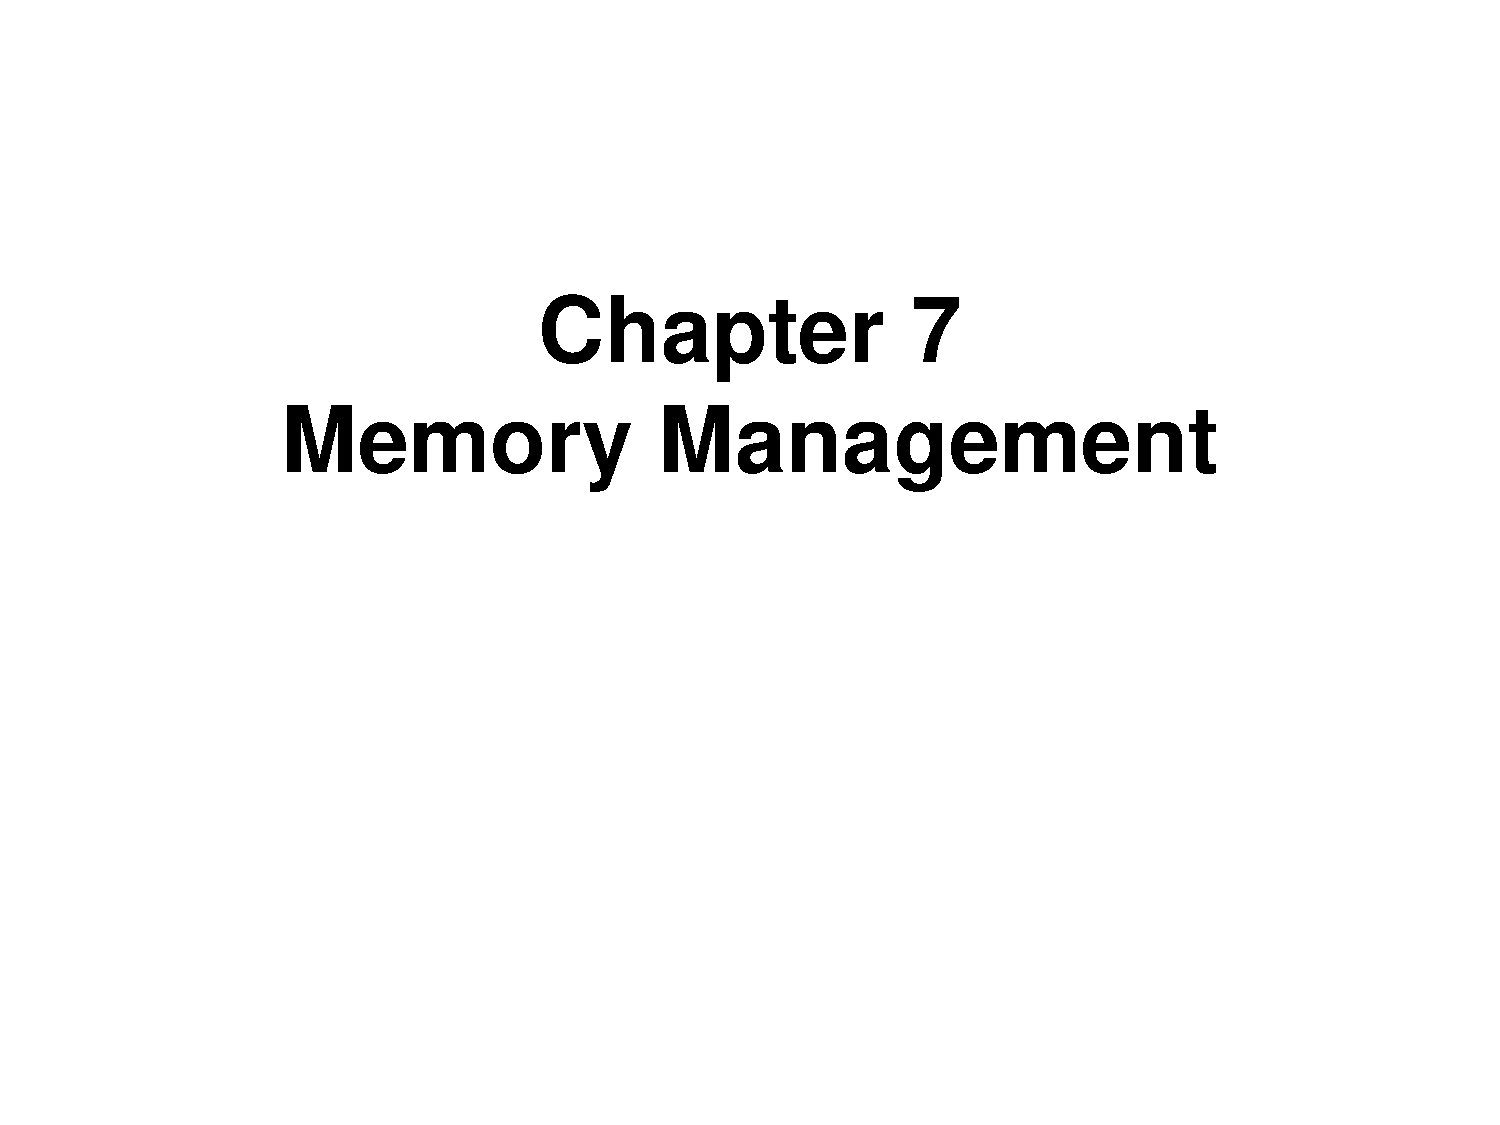
\includepdf[page=40]{07.pdf}
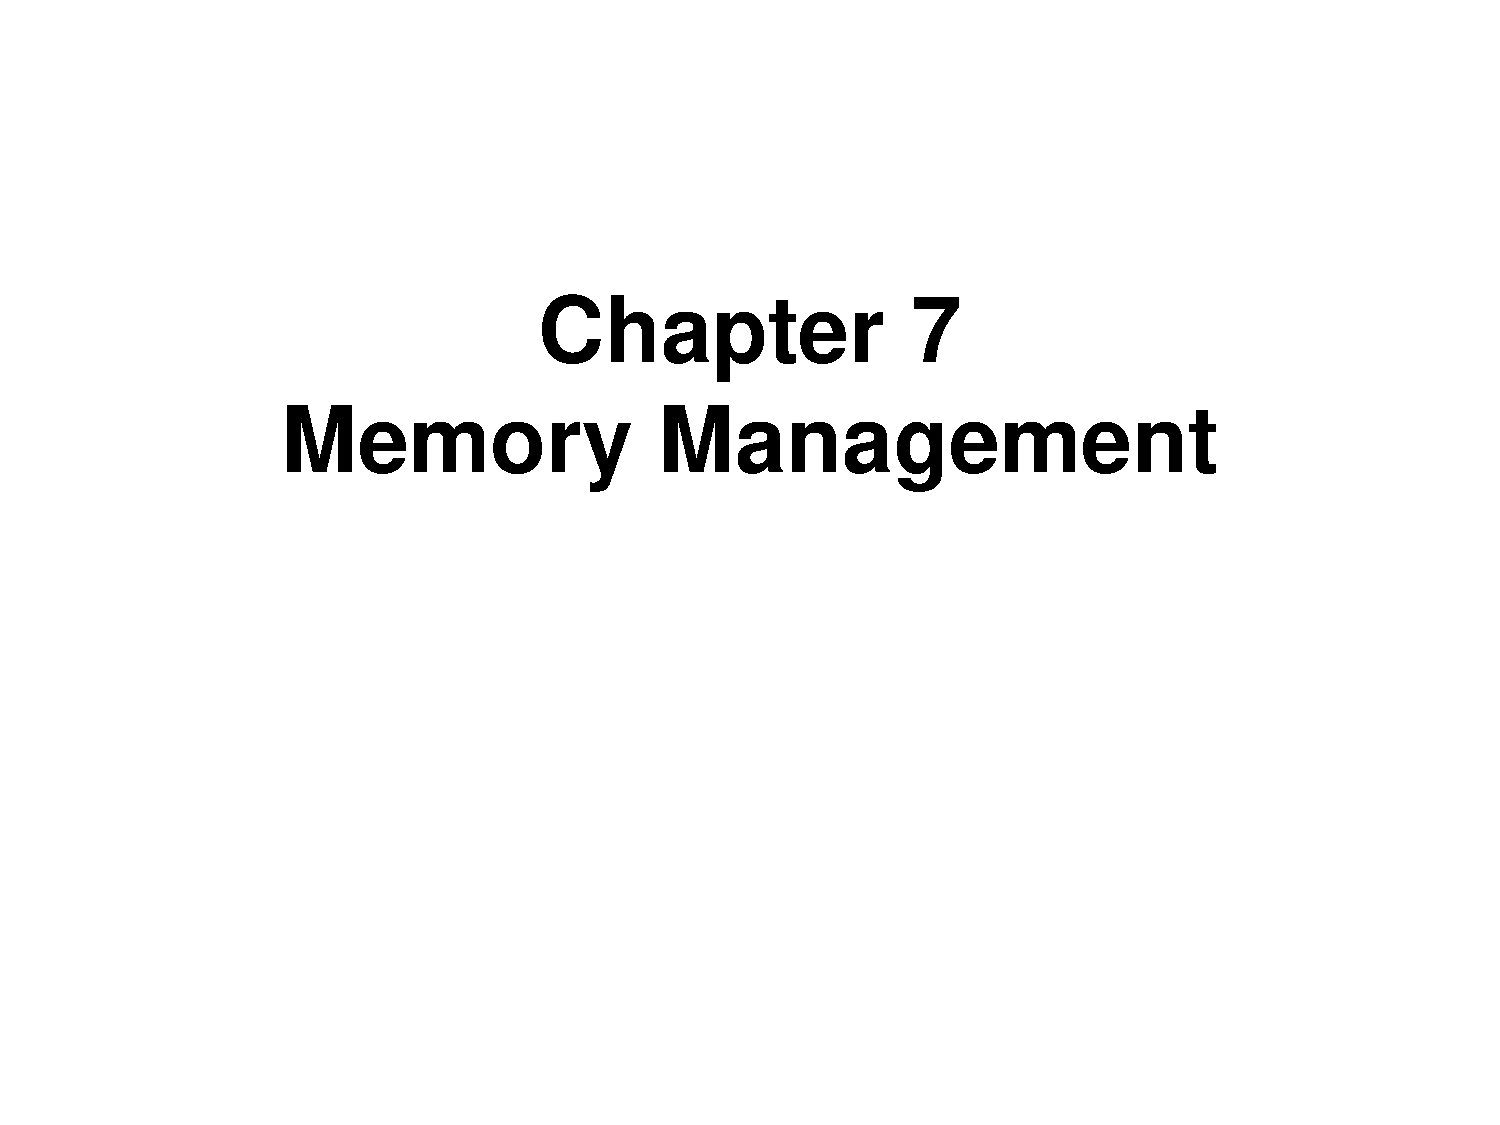
\includepdf[page=41]{07.pdf}

\end{document}
